\chapter{BASIC SCIENCE OF PLASMA-LIQUID SYSTEMS}
\label{chap:basic_science}

\Cref{chap:intro} outlined a few fundamental questions in plasma-liquids that had yet to be explored. These included:

\begin{itemize}
\item What's the role of convection in transport processes between plasma and liquid phases for discharges like coronas and jets?
\item How does varying interfacial parameters like the electron surface loss coefficient affect important plasma-liquid variables?
\item Why does decreasing solution conductivity increase the spreading of discharges over the liquid surface?
\end{itemize}

The role of convection is investigated in \cref{sec:plasfree_model}. Influence of interfacial parameters is considered in \cref{sec:plasliq}. While not explored in this dissertation, \cref{sec:plasliq} lays much needed groundwork for answering the third fundamental question of solution conductivity and discharge spreading.

\section{Momentum, Heat, and Neutral Mass Transport}
\label{sec:plasfree_model}

For a published version of much of the transport modelling work described in \cref{sec:plasfree_model}, the author encourages the reader to navigate to \cite{lindsay2015momentum}.

\subsection{Model Description}

The convective system chosen for modelling is shown in \cref{fig:streamer_picture}. It is essentially a point-to-plane pulsed-streamer in which the liquid surface serves as the gas discharge cathode. The streamer is self-pulsed because of a ballasting resistor; typical discharge voltages are between 6 and 8 kV and pulse frequencies are generally 10 to 30 kHz. The sharp anode tip can be stationed anywhere between 3 and 15 mm above the water surface. The water is contained within a glass petri dish of radius 3 cm; water treatment volumes are generally between 10 and 20 mL.

\begin{figure}[htpb]
    \centering
        \includegraphics[width=.5\textwidth]{streamer_picture_expt.eps}
        %\includegraphics[width=.5\textwidth]{streamer_picture_expt.jpg}
    \caption{Experimental set-up for pulsed streamer-liquid system. Discharge voltages are typically between 6 and 8 kV with pulse frequencies between 10 and 30 kHz. The gap from the needle tip to the water surface is between 3 and 15 mm. Water treatment volumes are between 10 and 20 mL.}
    \label{fig:streamer_picture}
\end{figure}

For the work in \cref{sec:plasfree_model}, we have chosen not to explicitly model the atmospheric discharge due to the computational cost of modeling of gas-liquid interfacial transport over time-scales of minutes (the equivalent of millions of individual pulses) using Comsol's seemingly inefficient plasma module. Instead, gas phase concentrations of the species modeled are taken from the DBD-water calculations in \cite{Tian2014} and diluted by a factor of 10; the gas phase species included and their respective inlet concentrations are shown in table \ref{tab:inletconc}. The factor 10 dilution is done for numerical stability.  High concentrations of reactive oxygen and nitrogen species (RONS) at the interface combined with very fast rate coefficients, particularly for reactions involving OH, can lead to singularities over our time scales of interest unless the computational mesh is sufficiently refined, requiring significant computational power. All concentration results and discussion will be focused on relative magnitudes and variation with space and time. The results in \cite{Tian2014} are chosen as an input basis because of the absence of experimental work for atmospheric plasmas in which a suite of gas-phase plasma species concentrations are reported. Most of the measurements in the literature focus on single species like OH \cite{ono1998measurement,ono2001oh,nakagawa2011density,verreycken2012time}, atomic oxygen \cite{niemi2005absolute}, or NO \cite{kanazawa2003two} that are accessible through Laser Induced Fluorescence (LIF).

A key feature of streamer discharges is the ionic wind. The ionic wind is a net flow of gas towards the cathode that results from the effective drag of cations on neutral gas molecules. In the streamer-liquid system studied, the ionic wind creates convective forces that affect species transport at the gas-liquid interface. Since the discharge is not modelled, another mechanism must be used to produce the ionic wind present in a streamer discharge. The mechanism chosen is a jet-like inlet with diameter equal to the diameter of the needle used in the experimental streamer set-up. The velocity profile at the inlet of the jet flow development channel is chosen such that the channel exit profile closely mimics that expected from streamer experiments and modeling. \cite{Zhao2005a} The profile is built from the expected streamer maximum axial velocity which is in turn determined from the work of Zhao et. al. Using values of 6 kV for the discharge voltage and 6.5 mm for the gap distance, the maximum axial velocity is interpolated to be 7.75 m/s near the needle tip. The spatial inlet profile is then computed from \cref{eq:v_in} assuming laminar no-slip conditions in the inlet channel: \cite{bird2007transport}

\begin{equation}
    v_{z} = v_{z,max}\left(1-\left(\frac{r}{R}\right)^2\right)
    \label{eq:v_in}
\end{equation}

 The model geometry is shown in \cref{fig:model_geom}; model inputs are summarized in \cref{tab:species_list,tab:gen_inputs,tab:henryconstants,tab:diffusioncoef,tab:inletconc}. The governing equations used to model the gas and liquid phases are the incompressible Navier-Stokes equations for momentum transport and convection-diffusion equations for heat and mass transport; they are shown in \cref{eq:mass_cont,eq:nav_stokes,eq:heat,eq:mass}

\begin{equation}
    \nabla\cdot\vec{u}=0
    \label{eq:mass_cont}
\end{equation}
\begin{equation}
    \rho \left(\frac{\partial\vec{u}}{\partial t}+\vec{u}\cdot\nabla\vec{u}\right)=-\nabla p+\mu \nabla^2 \vec{u}
    \label{eq:nav_stokes}
\end{equation}
\begin{equation}
    \rho C_p\vec{u}\cdot\nabla T = \nabla\cdot\left(k\nabla T\right)
    \label{eq:heat}
\end{equation}
\begin{equation}
    \nabla\cdot\left(-D_i\nabla C_i\right) + \vec{u}\cdot\nabla C_i = R_i
    \label{eq:mass}
\end{equation}

with $\vec{u}$ representing the fluid velocity, $\rho$ the overall mass density, p the static pressure, $\mu$ the dynamic viscosity, C$_p$ the constant pressure heat capacity, T the temperature, k the thermal conductivity, D$_i$ the diffusivity of species i, C$_i$ the concentration of species i, and R$_i$ the source term representing chemical reactions. When solving the model equations, the transient equations \ref{eq:mass_cont} and \ref{eq:nav_stokes} are solved until the velocity components and pressure reach a steady-state. Then the steady-state velocity field is inserted into the convection terms in equations \ref{eq:heat} and \ref{eq:mass}. The heat and mass transport equations are typically solved for a physical time of 1000 seconds in order to match common experimental treatment times in our laboratory. The temperature dependence of transport parameters in equations \ref{eq:heat} and \ref{eq:mass}, including reaction rate coefficients, is considered. Gaseous diffusion coefficients are assumed to scale with T$^{3/2}$ as predicted by Chapman-Enskog theory. \cite[p. 119]{cussler2009diffusion} The temperature dependence of liquid phase diffusion coefficients is constructed using the Stokes-Einstein equation \cite[p. 529]{bird2007transport} and the following equation for viscosity: \cite[p. 31]{bird2007transport}

\begin{equation}
	\mu \propto exp(3.8T_b/T)
	\label{eq:viscosityTempDependence}
\end{equation}

where T$_b$ is the boiling point of the solvent (373 K in the case of water). Reaction rate coefficients and their temperature dependence are contained in table \ref{tab:rxns}. Because the fluid flow equations are solved prior to solution of the heat transport equation, the temperature dependence of transport parameters in equations \ref{eq:mass_cont} and \ref{eq:nav_stokes} is not included in this work. Model boundary conditions are as follows: for fluid flow, all solid walls are assumed to be no-slip, i.e. all velocity components at the walls are zero. For most results presented the gas-liquid interface is assumed to be flat and static. For the static interface, the z-velocity component at the interface is set to zero in both the gas and liquid phases. Both the normal and shear stresses are continous across the interface. One may question whether the assumption of a flat interface is valid when in reality the interface is deformed by the gas flow. In the results section it will be demonstrated that for the purpose of this work, an assumption of a flat interfaction is sufficient. For temperature calculations, all solid surfaces are assumed to be insulated; at the interface, the temperature is assumed continuous. Additionally, evaporation of water at the surface is coupled to the system's heat transport in the following way: \cite{bird2007transport}

\begin{equation}
    Q_b = J_{z,H_2O}\cdot H_{vap} = -D_{H_2O,g}\cdot \left.\frac{\partial C_{H_2O(g)}}{\partial z}\right|_{z=interface}\cdot H_{vap}
    \label{eq:vapheatsrc}
\end{equation}

where Q$_b$ is the heat flux, J$_{z,H_2O}$ is the molar flux of H$_2$O coming from evaporation, and H$_{vap}$ is the latent heat of vaporization for water. The concentration of water vapor at the interface is determined from Antoine's equation: \cite{antoine1888thermodynamic}

\begin{equation}
    \log_{10}p = 8.07131 - \frac{1730.63}{233.426+T}
    \label{eq:Antoine}
\end{equation}

with p in units of mmHg, T in units of degrees Celsius, and the constant values taken from \cite{dimian2014integrated}.  The temperature at the gas inlet is set to 300 K for all times. Initially the temperature in both gas and liquid domains is 300 K. Inlet concentrations for species other than water vapor are specified at the beginnning of the jet flow development channel and are given in \cref{tab:inletconc}. Dilute species that are present in both gas and aqueous phases (OH, H$_2$O$_2$, NO, NO$_2$, N$_2$O$_4$, HNO$_2$, and HNO$_3$) have continuous fluxes across the gas-liquid interface. Concentrations immediately above and below the interface are assumed to be in equilibrium as described by their Henry's law coefficients, listed in \cref{tab:henryconstants}. A limited set of gas and liquid phase reactions encompassing the most important NO$_x$ chemistry is used to reduce computational expense. Even with this simplified reaction set and diluted concentration inputs, the simulation takes multiple days on a quad-core desktop and approaches 16 GB in required memory. As we move towards a more parallelizable software framework (see \cref{sec:plasliq} and \cref{chap:zapdos}), we plan to incorporate a more complete set of reacting species and reactions.  Some important species that were not included in this simplified set include oxygen and hydrogen radicals as well as water cluster ions to name a few. The reactions used in this study and their corresponding rate coefficients are listed in \cref{tab:rxns}. It should be noted that because of its highly acidic nature (pKa ~ -1.3), HNO$_3$ is assumed to dissociate into H$^+$ and NO$_3^-$ immediately after entering the aqueous phase. The model equations are solved using the finite element method implemented in Comsol Multiphysics version 4.4. A copy of the model is freely available upon request.

When the ``discharge region" is discussed, it is in reference to the gas region roughly demarcated in the z direction by the jet outlet/needle anode and the water surface, and in the radial direction by the radius of the jet channel/needle, where the plasma is visible during experiments. The reader is reminded that the plasma and its electrodynamics are not explicitly modeled in \cref{sec:plasfree_model}; the focus of this investigation is the qualitative behavior of momentum, heat, and neutral species mass transport in convective systems. The qualitative conclusions drawn here are equally applicable to atmospheric jets or streamer systems in which the ionic wind plays a key role in momentum transport. Moreover, we postulate that the steep gradients in highly reactive neutral species concentrations at the gas-liquid interface shown in the proceeding section are a universal phenomena of atmospheric plasma-liquid systems, regardless of whether they are convective or diffusive; this is consistent with the recent research by \cite{Chen2014a} as well as the greater reservoir of biochemistry literature \cite{Halliwell}. Morever, these gradients have important implications for plasma medicine, mainly that cellular responses must be induced through secondary as opposed to directly generated plasma reactivity.

\begin{figure}[htb]
    \centering
        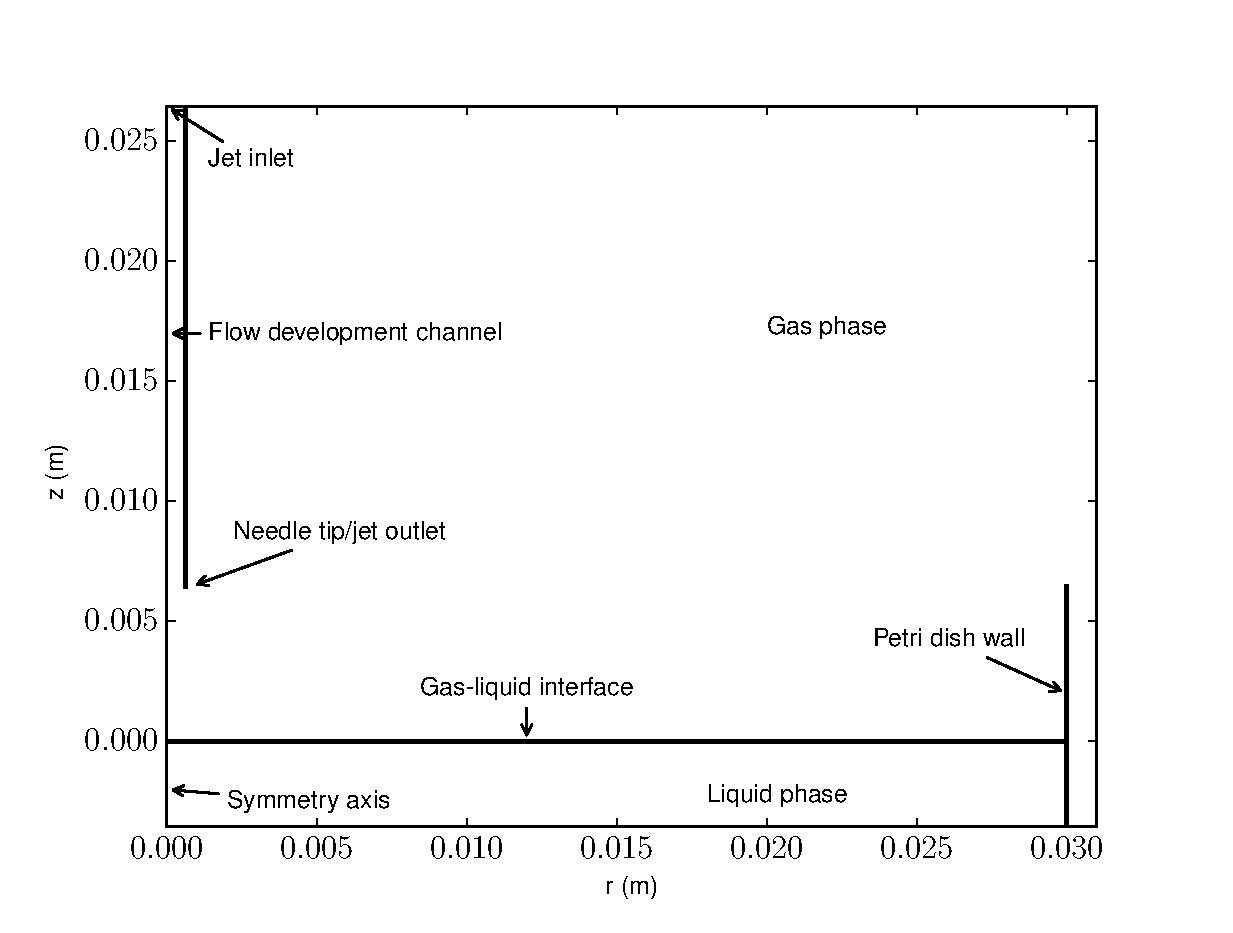
\includegraphics[width=\textwidth]{Geometry.eps}
        %\includegraphics[width=\textwidth]{Active_geometry_region.png}
    \caption{Experimental set-up for pulsed streamer-liquid system. Axis units are meters. The Python script used to create this figure, as well as the scripts used to create all subsequent figures can be found at \cite{scriptsLocation}}
    \label{fig:model_geom}
\end{figure}

\begin{table}[htpb]
    \begin{center}
        \begin{tabular}{|l| p{10cm}|}
            \hline
            Gas phase species & OH, H$_2$O$_2$, NO, NO$_2$, N$_2$O$_4$, HNO$_2$, HNO$_3$, H$_2$O \\
            \hline
            Liquid phase species & OH, H$_2$O$_2$, NO, NO$_2$, N$_2$O$_4$, HNO$_2$, NO$_2^-$, NO$_3^-$, ONOOH, H$^+$, OH$^-$ \\
            \hline
        \end{tabular}
    \end{center}
    \caption{Species included in the model}
    \label{tab:species_list}
\end{table}


\begin{table}[htpb]
    \begin{center}
        \begin{tabular}{|c |c |}
        \hline
        Needle diamater & 1.2 mm \\
        \hline
        Petri dish diameter & 6 cm \\
        \hline
        Gap distance & 6.5 mm \\
        \hline
        Water volume & 10 mL \\
        \hline
        Jet channel length & 2 cm \\
        \hline
        Maximum axial velocity of ionic wind/jet & 7.75 m/s \\
        \hline
        \end{tabular}
    \end{center}
    \caption{General model inputs}
    \label{tab:gen_inputs}
\end{table}

%\begin{minipage}[t]{0.25\textwidth}
    \begin{table}[htpb] %[H]
        \begin{center}
            \begin{tabular}{c |c }\rmfamily
                Molecule & H$_i$ [unitless] \\ \hline \hline
                OH & $6.92\cdot10^2$\\
                H$_2$O$_2$ & $1.92\cdot10^6$\\
                NO & $4.4\cdot10^{-2}$\\
                NO$_2$ & $2.8\cdot10^{-1}$\\
                N$_2$O$_4$ & $3.69\cdot10^1$\\
                HNO$_2$ & $1.15\cdot10^3$\\
                HNO$_3$ & $4.8\cdot10^6$\\
                HOONO & $4.8\cdot10^6$\\
            \end{tabular}
    \end{center}
        \caption{The Henry's constant for a number of molecules\cite{Tian2014}.}
        \label{tab:henryconstants}
    \end{table}
%\end{minipage}

%\begin{minipage}[t]{0.1\textwidth}
 %   \hspace{1cm}
%\end{minipage}

%\begin{minipage}[t]{0.25\textwidth}
    \begin{table}[htpb] %[H]
        \begin{center}
            \begin{tabular}{c |c |c}\rmfamily
                Molecule & D [m$^2$ s$^{-1}$]& reference\\ \hline \hline
                OH(g) & $4\cdot10^{-5}$ & \cite{Sakiyama2012b}\\
                H$_2$O$_2$(g) & $2\cdot10^{-5}$ & \cite{Sakiyama2012b}\\
                NO(g) & $2\cdot10^{-5}$ & \cite{Sakiyama2012b}\\
                NO$_2$(g) & $1.7\cdot10^{-5}$ & \cite{Sakiyama2012b}\\
                N$_2$O$_4$(g) & $1\cdot10^{-5}$ & \cite{Sakiyama2012b}\\
                HNO$_2$(g) & $2.1\cdot10^{-5}$ & \cite{Sakiyama2012b}\\
                HNO$_3$(g) & $2.1\cdot10^{-5}$ & \cite{Sakiyama2012b}\\
                H$_2$O(g) & $2.3\cdot10^{-5}$ & \cite{Sakiyama2012b}\\
                OH(aq) & $2.8\cdot10^{-9} [310 K]$ & \cite{khalack2005solvation}\\
                H$_2$O$_2$(aq) & $1.7\cdot10^{-9}$ & \cite{mcmurtrie1948measurement}\\
                NO(aq) & $2.2\cdot10^{-9}$ & \cite{zacharia2005diffusivity}\\
                NO$_2$(aq) & $1.85\cdot10^{-9} [296 K]$ & \cite{skinn2013nitrogen}\\
                N$_2$O$_4$(aq) & $1.5\cdot10^{-9}$ & Estimate\\
                HNO$_2$(aq) & $2.5\cdot10^{-9}$ & By analogy with nitric acid\\
                HNO$_3$(aq) & $2.5\cdot10^{-9}$ & \cite{wills1971diffusion}\\
                ONOOH(aq) & $2.5\cdot10^{-9}$ & By analogy with nitric acid\\
                NO$^{-}_2$(aq) & $1.7\cdot10^{-9}$ & \cite{kreft2001individual}\\
                NO$^{-}_3$(aq) & $1.7\cdot10^{-9}$ & \cite{kreft2001individual}\\
                H$^{+}$(aq) & $7\cdot10^{-9}$ & \cite{agmon1995grotthuss}\\
                OH$^{-}$(aq) & $5.29\cdot10^{-9}$ & \cite{kitamura1994microchemistry}\\
            \end{tabular}
        \end{center}
        \caption{The diffusion coefficients for a number of molecules at 300 K. See text for implementation of temperature dependence.}
        \label{tab:diffusioncoef}
    \end{table}
%\end{minipage}

\begin{table}[htpb]
    \begin{center}
        \begin{tabular}{c |c}\rmfamily
           Molecule & Molecule inlet concentration [m$^{-3}$]\\ \hline \hline
            OH & $1.3\cdot10^{18}$ \\
            H$_2$O$_2$ & $1.6\cdot10^{17}$ \\
            NO & $8\cdot10^{18}$ \\
            NO$_2$ & $5\cdot10^{16}$ \\
            N$_2$O$_4$ & 0 \\
            HNO$_2$ & $8\cdot10^{17}$ \\
            HNO$_3$ & $9\cdot10^{16}$ \\
            H$_2$O & 0 \\
        \end{tabular}
    \end{center}
    \caption{Gaseous species inlet concentrations. \cite{Tian2014} See text for discussion}
    \label{tab:inletconc}
\end{table}

\begin{table}[htpb]
    \begin{center}
        \begin{tabular}{l |p{6cm} |p{3cm}}\rmfamily
            Reaction & Rate coefficient (Units of s$^{-1}$, m$^3$ mol$^{-1}$ s$^{-1}$, or m$^6$ mol$^{-2}$ s$^{-1}$. Temperature in K. Concentration of M in gas and H$_2$O in liquid are lumped into rate coefficient) & Reference \\ \hline \hline
            Gas phase reactions \\
            1. 2NO$_2 \rightarrow$ N$_2$O$_4$ & $6.02\cdot10^5\cdot(300/T)^{3.8}$ & \cite{Sakiyama2012b} \\
            2. N$_2$O$_4 \rightarrow$ 2NO$_2$ & $4.4\cdot10^6\cdot\exp(-4952/T)$ & \cite{Sakiyama2012b} \\
            3. NO + OH + M $\rightarrow$ HNO$_2$ + M & $1.1\cdot10^{7}\cdot(300/T)^{2.4}$ & \cite{Sakiyama2012b} \\
            4. NO + NO$_2$ + H$_2$O $\rightarrow$ 2HNO$_2$ & 22 & \cite{wayne1951kinetics} \\
            5. 2OH + M $\rightarrow$ H$_2$O$_2$ + M & $1.0\cdot10^7\cdot(T/300)^{-0.8}$ & \cite{Sakiyama2012b} \\
            6. NO$_2$ + OH + M $\rightarrow$ HNO$_3$ + M & $3.2\cdot10^7\cdot(300/T)^{2.9}$ & \cite{Sakiyama2012b} \\
            7. OH + HNO$_2$ $\rightarrow$ NO$_2$ + H$_2$O & $3.0\cdot10^6\cdot\exp(-390/T)$ & \cite{Sakiyama2012b} \\
            8. 2HNO$_2$ $\rightarrow$ NO + NO$_2$ + H$_2$O & $6.0\cdot10^{-3}$ & \cite{Sakiyama2012b} \\
            9. HNO$_2$ + HNO$_3$ $\rightarrow$ 2NO$_2$ + H$_2$O & 9.6 & \cite{Sakiyama2012b} \\
            10. HNO$_3$ + NO $\rightarrow$ HNO$_2$ + NO$_2$ & $4.4\cdot10^{-3}$ & \cite{dorai2002modeling} \\
            \\
            Liquid phase reactions \\
            11. N$_2$O$_4$ + H$_2$O $\rightarrow$ NO$_2^-$ + NO$_3^-$ + 2H$^+$ & 1000 & \cite{coddington1999hydroxyl} \\
            12. 2NO$_2$ + H$_2$O $\rightarrow$ NO$_2^-$ + NO$_3^-$ + 2H$^+$ & $8.4\cdot10^{4}\cdot\exp(-0.033\cdot(T-295))$ & \cite{park1988solubility} \\
            13. NO + NO$_2$ + H$_2$O $\rightarrow$ 2NO$_2^-$ + 2H$^+$ & $1.6\cdot10^{5}$ & \cite{park1988solubility} \\
            \ONOOHlong{}. NO$_2^-$ + H$_2$O$_2$ + H$^+$ $\rightarrow$ ONOOH + H$_2$O & $1.1\cdot10^{-3}$ & \cite{Lukes2014b}\\
            \OHfromONOOH{}. ONOOH $\rightarrow$ .7(NO$_3^-$ + H$^+$) + .3(NO$_2$ + OH) & .8 & \cite{coddington1999hydroxyl}\\
            \ONOOHshort{}. NO$_2$ + OH $\rightarrow$ ONOOH & $5.3\cdot10^{6}$ & \cite{Lukes2014b,goldstein2005chemistry}\\
            17. 2OH + M $\rightarrow$ H$_2$O$_2$ + M & $1\cdot10^{7}\cdot\exp(-450\cdot(1/T-1/298))$ & \cite{johnaelliot1990estimation}\\
            18. HNO$_2$ $\rightarrow$ H$^+$ + NO$_2^-$ & $3.51\cdot10^{6}$ & From reaction \NitrousAcidAssociation{} and equilibrium constant \\
            \NitrousAcidAssociation{}. H$^+$ + NO$_2^-$ $\rightarrow$ HNO$_2$ & $7\cdot10^{6}$ & Assumes diffusion limited\\
            \WaterAssociation{}. H$^+$ + OH$^-$ $\rightarrow$ H$_2$O & $7\cdot10^{6}$ & Assumes diffusion limited \\
            21. H$_2$O $\rightarrow$ H$^+$ + OH$^-$ & $7\cdot10^{-2}$ & From reaction \WaterAssociation{} and equilibrium constant\\
            22. NO + OH $\rightarrow$ HNO$_2$ & $2\cdot10^{7}$ & \cite{Tian2014}\\
			23. 2HNO$_2$ $\rightarrow$ NO + NO$_2$ & $1.34\cdot10^{-2}\cdot\exp(.106\cdot(T-295))$ & \cite{park1988solubility}
        \end{tabular}
    \end{center}
    \caption{Reactions considered in model}
    \label{tab:rxns}
\end{table}

\subsection{Results and Discussion}

The steady state velocity field is shown in figure \ref{fig:v_field}. The recirculating pattern observed in the gas phase is consistent with the corona discharge modelling results reported in \cite{Zhao2005a}. A similar recirculation pattern is observed in the liquid phase, induced by shear stresses between the phases at the gas-liquid interface. The maximum liquid phase velocity, .1 m/s, occurs along the interface approximately .8 mm away from the stagnation point (r = 0).

\begin{figure}[htb]
    \centering
        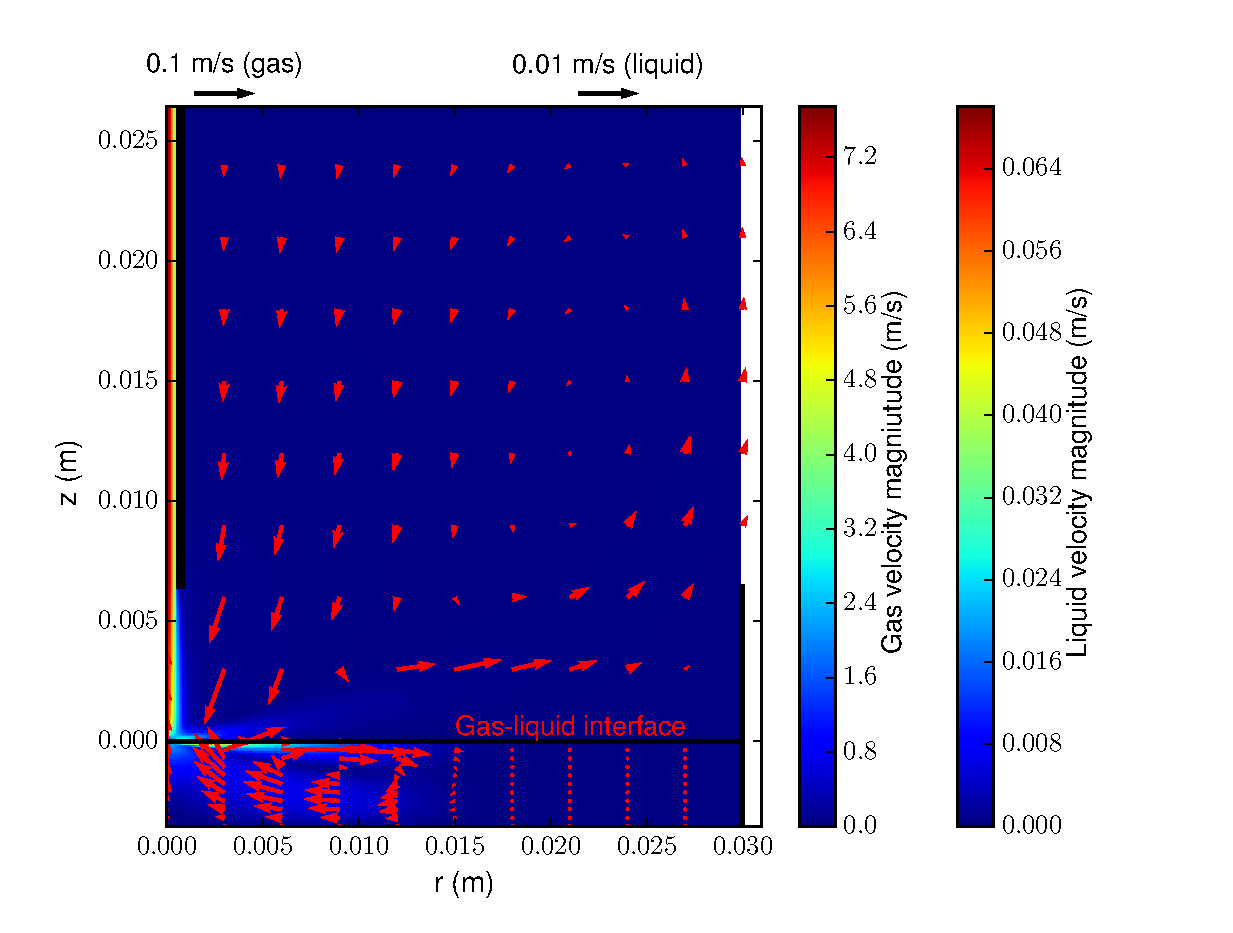
\includegraphics[width=\textwidth]{velocity.eps}
        %\includegraphics[width=\textwidth]{Fluid_flow.jpg}
    \caption{Velocity magnitude and direction. Axis units are meters. Interface is at z = 0. Axis of symmetry is at r = 0. Selected velocity vectors are overlaid on color scale indicating velocity magnitude. Red color represents higher values and blue color represents lower values. Velocity vector arrows are scaled 12.5 times larger in the aqueous phase.}
    \label{fig:v_field}
\end{figure}

The temperature and water vapor profiles at the end of the simulation (t = 1000 seconds) are shown in figures \ref{fig:temp_2D_profile} and \ref{fig:water_2D_profile}. Notably, the temperature in the bulk liquid has fallen close to 10 K from its initial value of 300 K. This drop in temperature in the bulk liquid is an example of the classical wet-bulb/dry-bulb problem found in chemical engineering texts. Water vapor present in the gas above the interface is whisked away by convection. In order to maintain the equilibrium vapor pressure required by Antoine's equation, liquid water must be evaporated, consuming heat and lowering the temperature at the interface. Heat then migrates from the bulk liquid to the surface, leading to bulk liquid cooling. In this problem we have assumed that the impinging gas is at room temperature, and subsequently convection-induced evaporation leads to cooling of the bulk liquid below room ambient. However, if there is significant plasma heating of the gas, it is possible that heating of the liquid above the initial temperature will be observed experimentally. The important point is that the natural coupling between heat transport and evaporation leads to significant spatial variation in temperature, particularly at the interface, and a cooling of the bulk liquid relative to the gas. An example of the steep temperature gradients is shown in figure \ref{fig:temp_1D_profile} where the gas phase temperature changes by 10 K over the span of 200 $\mu$m, immediately above the liquid surface. Because reaction rates typically exhibit Arrhenius dependence on temperature, physical factors that introduce steep temperature gradients should be included in any model that wishes to accurately predict plasma-liquid chemistry. Though not shown here, a simulation was conducted in which temperature and water-vapor transport were de-coupled and the interfacial temperature gradient removed. Compared to the coupled case, concentrations of long-lived aqueous species like H$_2$O$_2$, NO$_2^-$, and NO$_3^-$ differed by as large as factors of two at the end of the simulation, demonstrating the importance of accounting for evaporation-induced temperature gradients.

Another instance of transport coupling that may impact plasma-liquid chemistry is the significant radial gradients in the concentration of water vapor between the needle tip/jet outlet and gas-liquid interface. An example of these gradients induced by convective forces are shown in figure \ref{fig:water_1D_profile}. Examining the dotted curve, which gives the radial distribution of water vapor half-way between the jet outlet/needle tip and liquid surface, one can see that the water vapor concentration drops precipitously in the region of the discharge (r $<$ 2 mm). In the center of the discharge (r $=$ 0) the water vapor concentration is essentially zero. This large drop in the concentration of water vapor in the active discharge region due to convection suggests that the concentrations of plasma species which rely on H$_2$O as a precursor will be reduced at increasing distances from the liquid surface, relative to  discharges where diffusion is the dominant mechanism of mass transport.

\begin{figure}[htb]
    \centering
        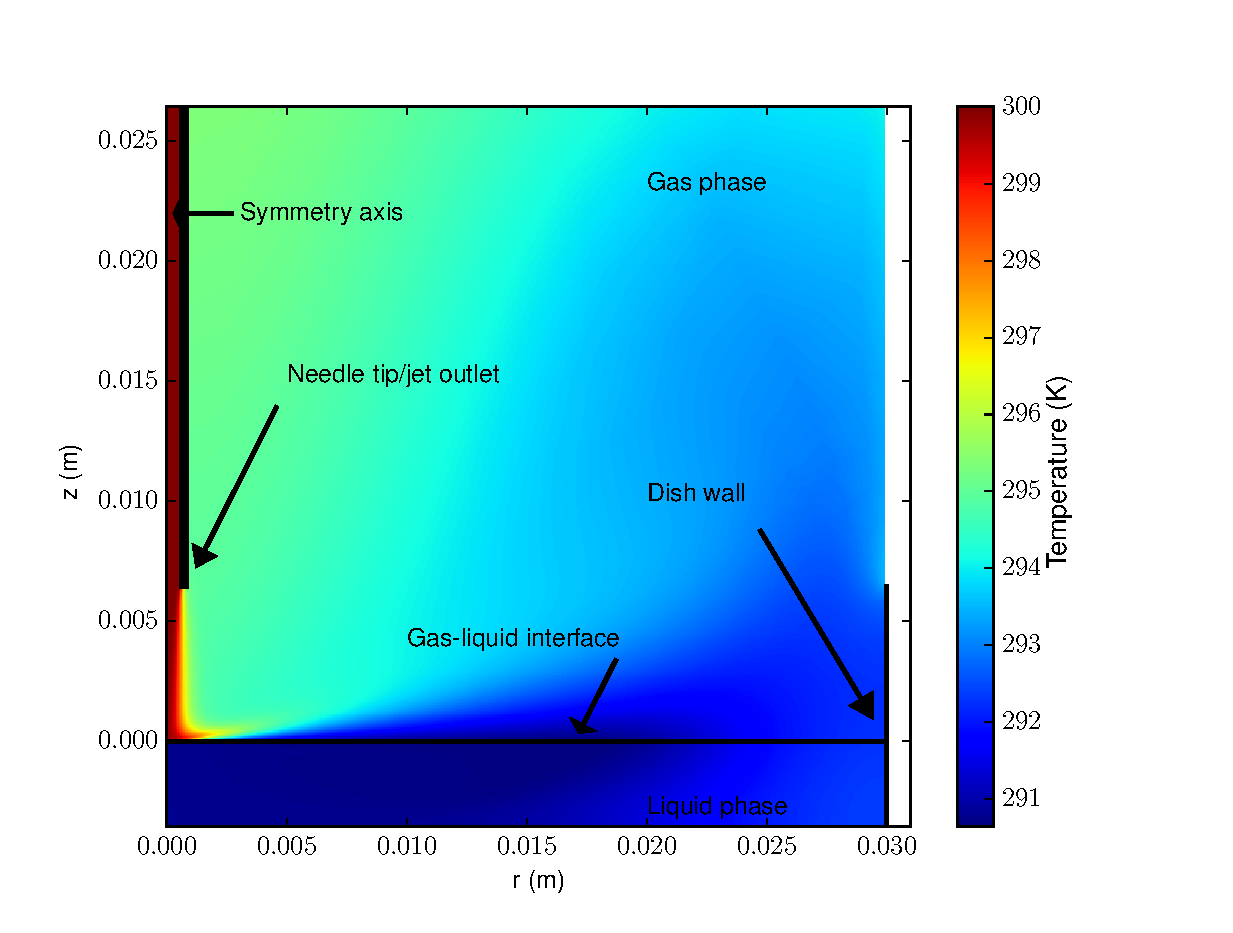
\includegraphics[width=\textwidth]{Temperature2D.eps}
        %\includegraphics[width=\textwidth]{Temperature.jpg}
        \caption{2D temperature profile at t = 1000 seconds. Red color represents higher values; blue color lower values. Inlet temperature is 300 K. Temperature in the bulk liquid has cooled by approximately 10 K because of convection-induced evaporative cooling.}
        \label{fig:temp_2D_profile}
\end{figure}

\begin{figure}[htb]
    \centering
        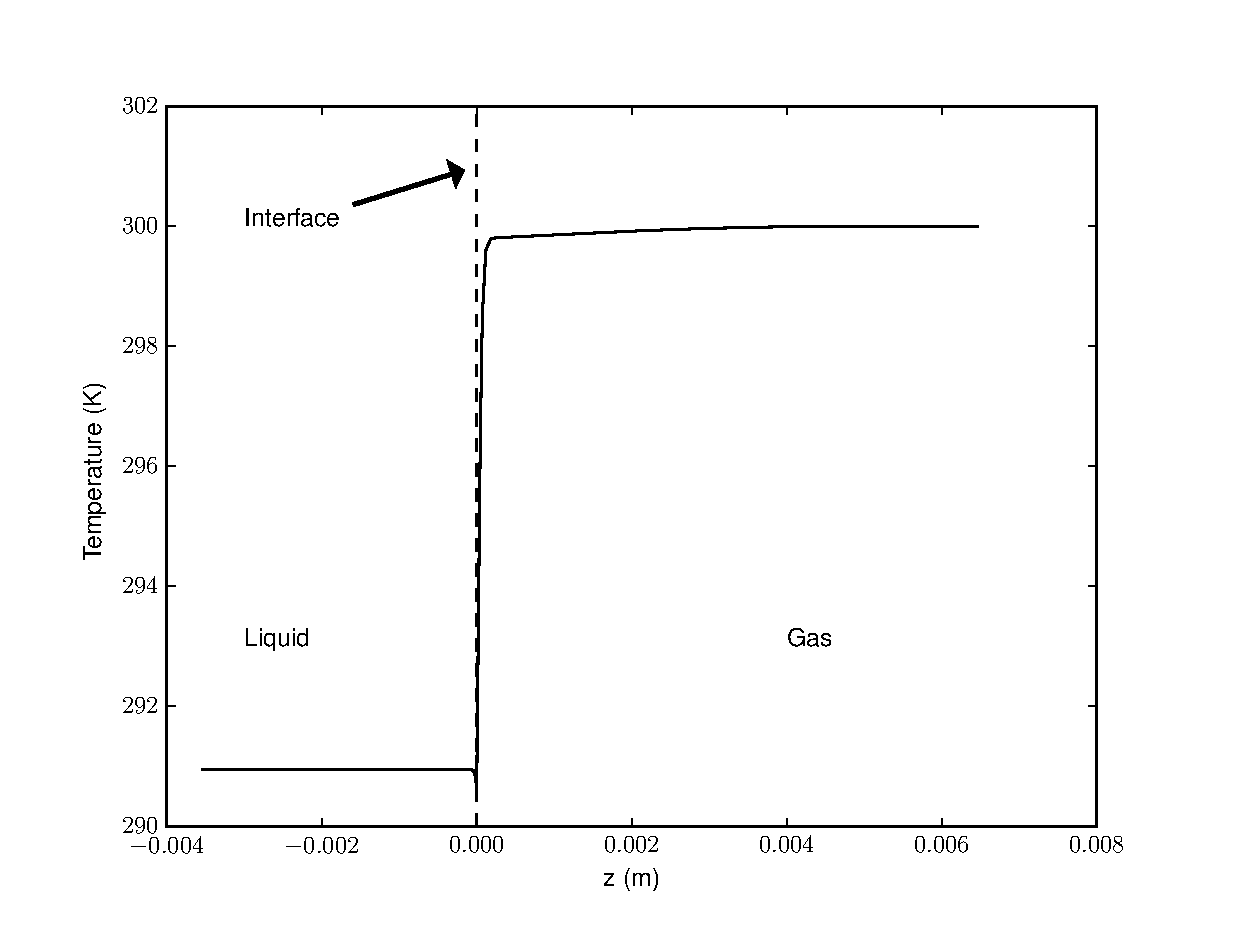
\includegraphics[width=\textwidth]{1D_temperature_plot.eps}
        \caption{Temperature along z-axis. Illustrates the large temperature gradient that exists at the gas-liquid interface and the resulting difference in bulk gas and liquid temperatures.}
        \label{fig:temp_1D_profile}
\end{figure}

\begin{figure}[htb]
    \centering
        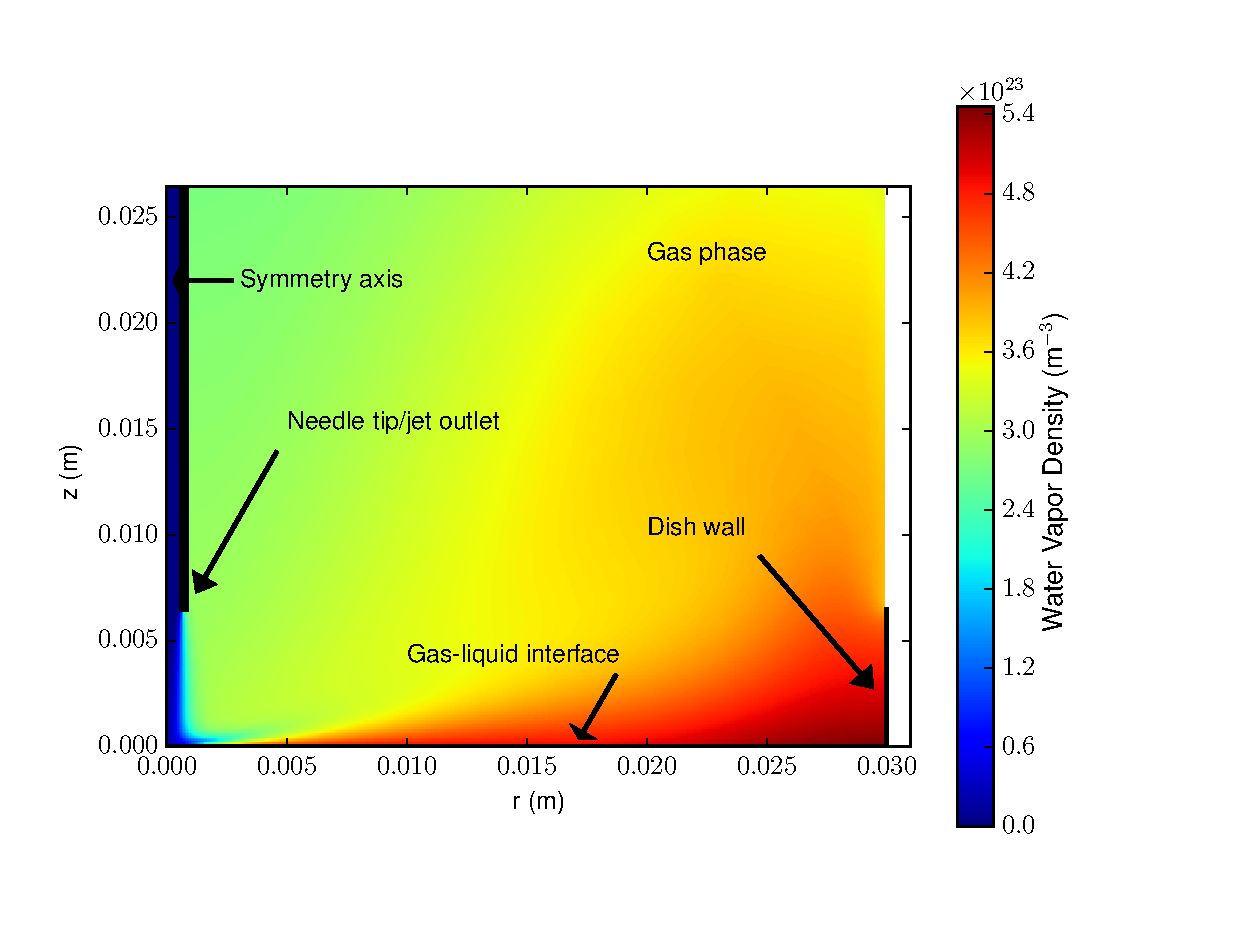
\includegraphics[width=\textwidth]{WaterVapor2D.eps}
        %\includegraphics[width=\textwidth]{Water_vapor.jpg}
        \caption{2-D water vapor profile at t = 1000 seconds. Red color represents higher values of water vapor concentration; blue color lower values. As implemented through Antoine's equation, water vapor concentration at the interface is highest where the temperature is highest. Role of convection in water vapor profile is evident in decreased concentration near the streamer/jet.}
        \label{fig:water_2D_profile}
\end{figure}


\begin{figure}[htb]
    \centering
        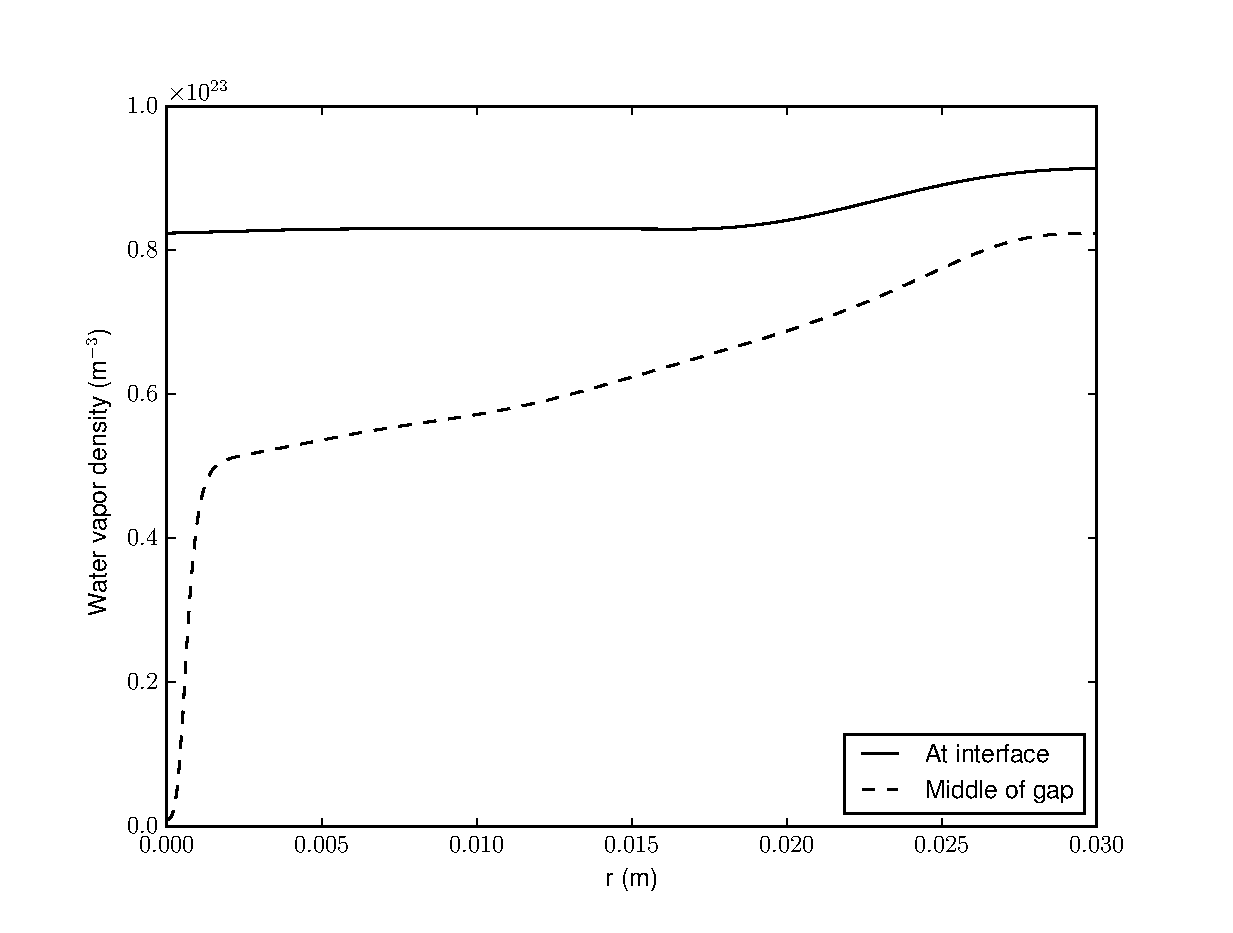
\includegraphics[width=\textwidth]{1D_water_vapor_plot.eps}
        \caption{Radial water vapor profiles. Horizontal axis is the radial coordinate. The top curve (solid) corresponds to the water vapor concentration at the interface. The bottom curve (dashed) shows the strong water vapor radial dependence in the middle of the streamer/jet gap. Gradient is largest near and inside the discharge region.}
        \label{fig:water_1D_profile}
\end{figure}

This model also addresses the role that convection plays in dissolution rates of different gaseous species. For this analysis, reactions are turned off, reducing mass transport to only convection and diffusion. As one might intuitively expect, the induced convective flow in the liquid significantly changes the spatial distribution of aqueous species relative to a diffusion only case, as demonstrated for HNO$_3$ in figures \ref{fig:HNO3_convec} and \ref{fig:HNO3_diffus} (note that gas convection is present in both figures). However, what is perhaps not intuitive is that though the HNO$_3$ spatial distribution changes dramatically depending on whether convection is present in the liquid, the volume-averaged uptake of HNO$_3$ does not change from diffusion-dominated to convection-dominated cases as shown in figure \ref{fig:HNO3_mass_compare}. If a hydrophobic specie like NO is examined instead of a hydrophilic specie like HNO$_3$, it is observed that the presence of liquid convection increases volume-averaged uptake significantly, as illustrated in figure \ref{fig:NO_mass_compare}. This fundamental difference in behavior between hydrophilic and hydrophobic species can be explained in terms of lumped mass transfer resistances. For a hydrophilic specie, the dominant resistance to interfacial transfer is in the gas-phase, whereas for a hydrophobic specie the dominant resistance to transfer occurs in the liquid phase. \cite[p. 249]{carberry2001chemical} Consequently, when convection is added to the liquid phase, effectively reducing the liquid-side mass transfer resistance, the overall resistance to mass transfer decreases and the volume-averaged uptake increases significantly for hydrophobic species like NO whereas the change in overall resistance is miniscule for hydrophilic species like HNO$_3$.

\begin{figure}[htpb]
    \centering
    \begin{subfigure}[b]{.7\textwidth}
        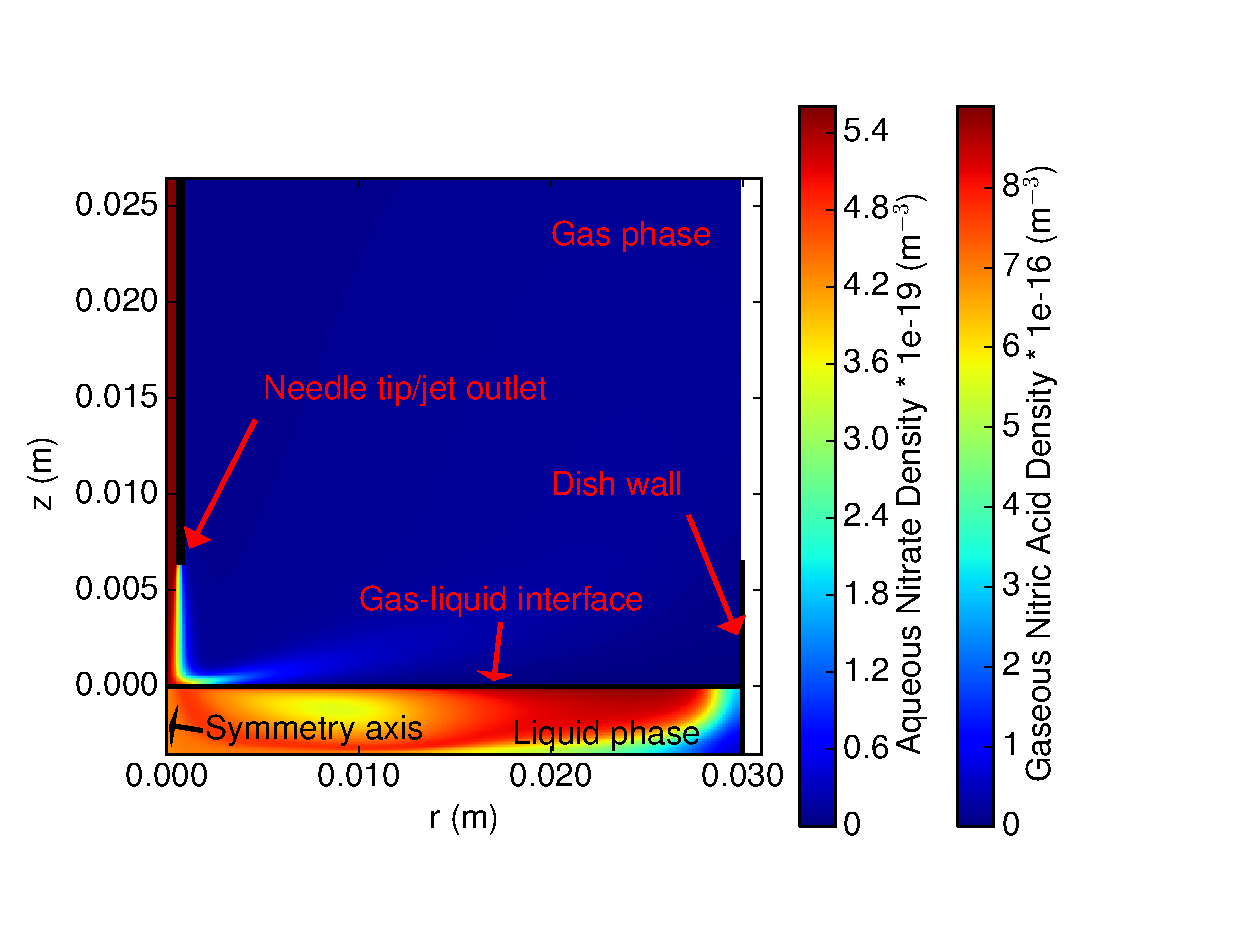
\includegraphics[width=\textwidth]{HNO3Convection2D.eps}
        \caption{Distribution of HNO$_3$ with liquid convection turned on. t = 1000 s}
        \label{fig:HNO3_convec}
    \end{subfigure}
    %\quad
    \begin{subfigure}[b]{.7\textwidth}
        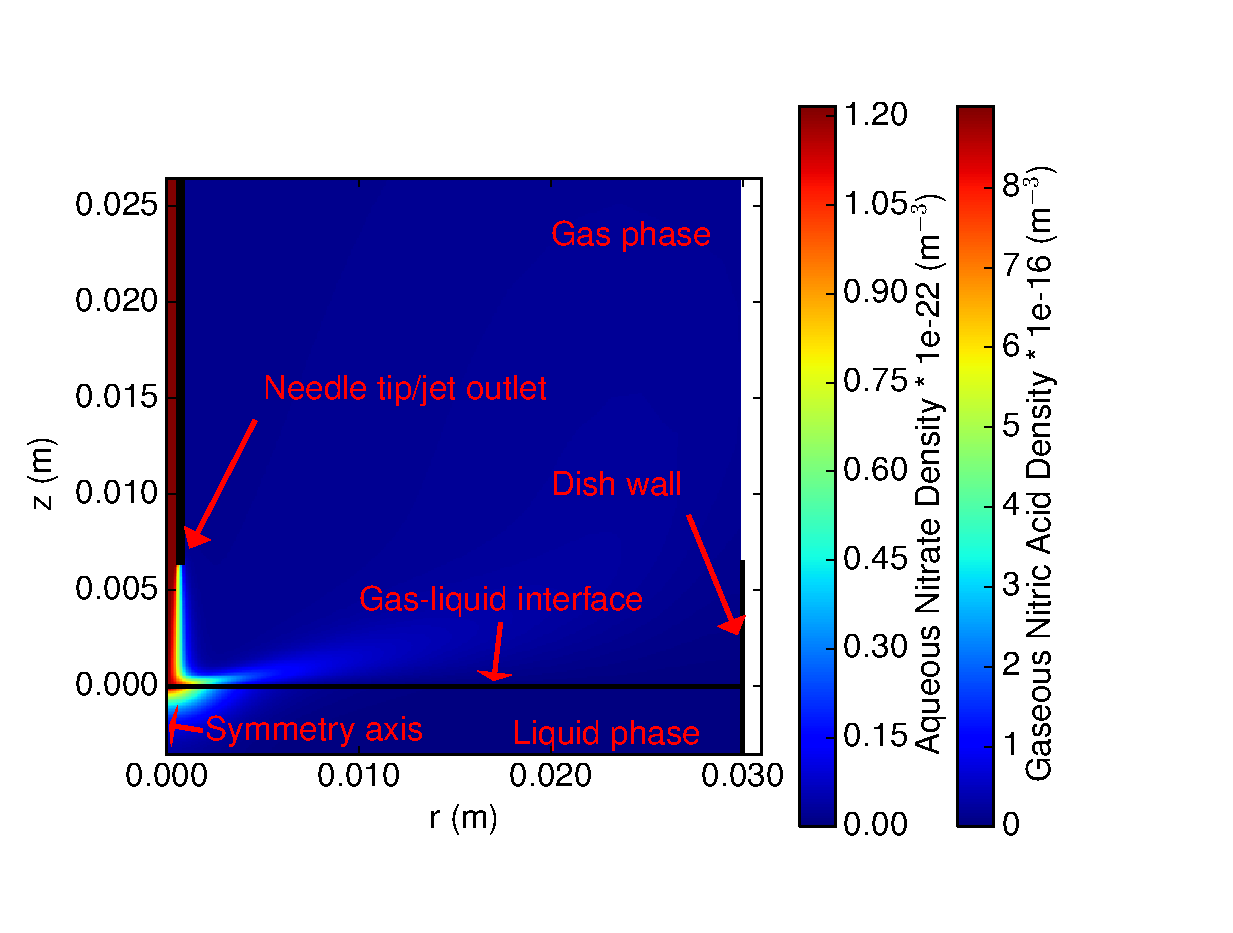
\includegraphics[width=\textwidth]{HNO3Diffusion2D.eps}
        \caption{Distribution of HNO$_3$ with liquid convection turned off. t = 1000 s}
        \label{fig:HNO3_diffus}
    \end{subfigure}
    \caption{}
    \label{fig:HNO3}
\end{figure}

\begin{figure}[htpb]
    \centering
    \begin{subfigure}[b]{.63\textwidth}
        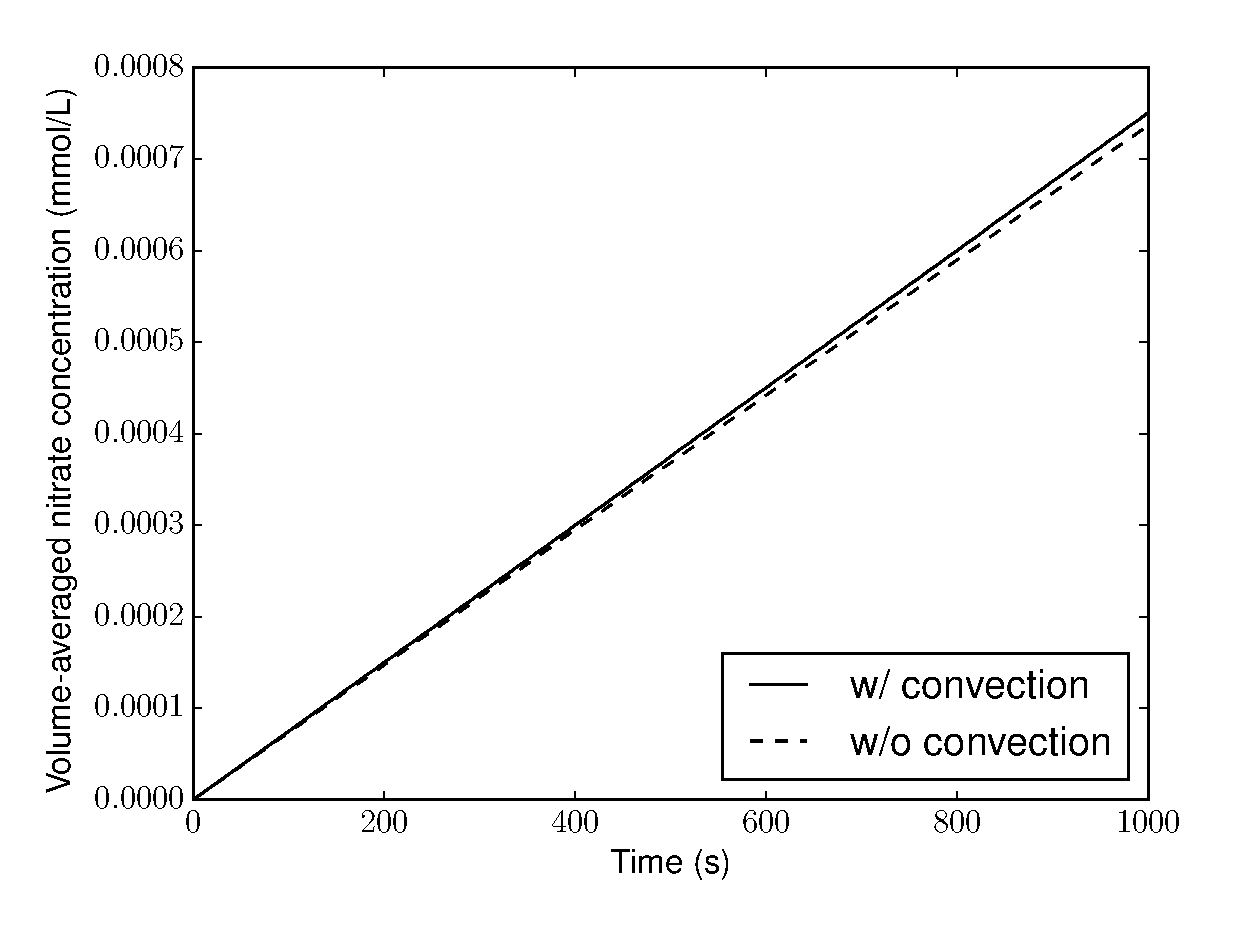
\includegraphics[width=\textwidth]{Nitrate_uptake_plot.eps}
        \caption{Comparison of volume averaged uptake of nitrate (HNO$_3$ before dissolution) with liquid convection toggled on or off. Very little difference between the two cases.}
        \label{fig:HNO3_mass_compare}
    \end{subfigure}
    %\quad
    \begin{subfigure}[b]{.63\textwidth}
        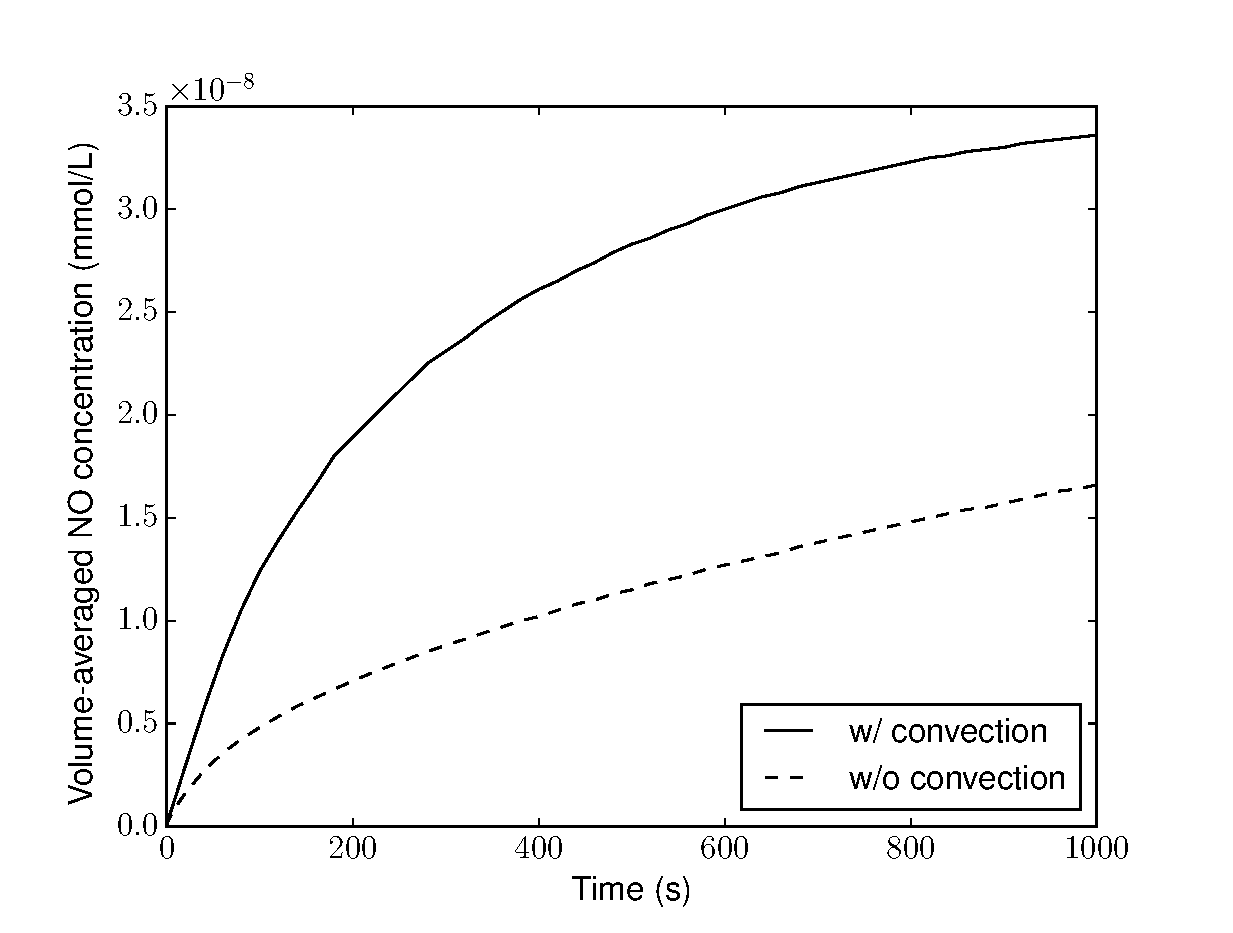
\includegraphics[width=\textwidth]{NO_uptake_plot.eps}
        \caption{Comparison of volume averaged uptake of NO with liquid convection toggled on or off. The presence of convection increases the volume-averaged concentration by roughly a factor of 2 over the course of the simulation. Note that the vertical scale is much smaller for NO than for HNO$_3$ in \ref{fig:HNO3_mass_compare} because of NO's hydrophobicity}
        \label{fig:NO_mass_compare}
    \end{subfigure}
    \caption{}
    \label{fig:excel}
\end{figure}

When the full reaction set is considered, large gradients in reactive species concentrations emerge at the interface. Of particular interest for biomedical or pollutant degradation applications is the distribution of hydroxyl radical in the aqueous phase. Figure \ref{fig:log_OH_conc} shows a 3D plot of the base 10 log of OH(aq) concentration versus radial and axial position for t = 1000 seconds. Interfacial gradients in OH concentration are prominent in the region where the discharge impinges on the water surface. At the stagnation point (r=0) the OH concentration drops by approximately 9 orders of magnitude over the span of 50 $\mu$m in the axial direction. Moving away from where the streamer/jet touches the surface, the interfacial gradients become less pronounced. Even so, the largest OH concentration away from the surface and in the bulk solution is 3-4 orders of magnitude lower than the peak OH concentration which occurs at the interface and at the center of the impinging streamer/jet. The presence of the liquid phase convective loop is evident from the OH concentration hole in the center of Figure \ref{fig:log_OH_conc}. The effect is also seen in the center of Figure \ref{fig:log_ONOOH_conc} for ONOOH.

\begin{figure}[htb]
    \centering
    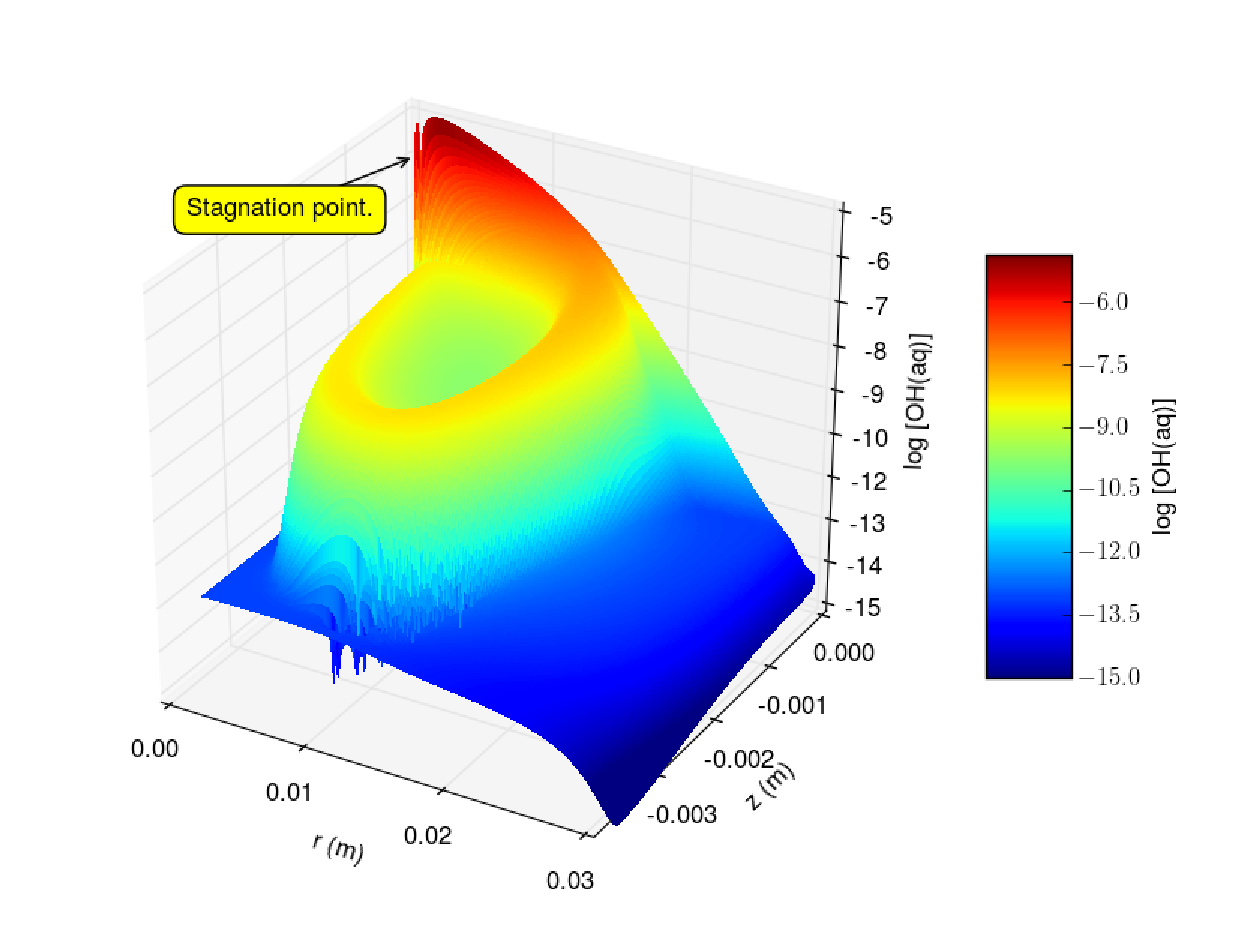
\includegraphics[width=\textwidth]{logOH.eps}
    \caption{3D plot of log$_{10}$(OH(aq)) as a function of position for t = 1000 seconds. Large interfacial gradients are evident, particularly at the stagnation point (r=z=0). Note the effect of convection in the hole in OH concentration in the center of the plot. Some numerical noise is observed at very low OH concentrations towards the bottom of the dish. Note that the r and z axes have different scales}
    \label{fig:log_OH_conc}
\end{figure}

Another plasma-generated specie which has received much attention in the literature is peroxynitrous acid and its conjugate base peroxynitrite. In the current model, ONOOH exists only in the liquid phase and can be created through two mechanisms: reactions \ONOOHlong{} and \ONOOHshort{} in table \ref{tab:rxns}. Reaction \ONOOHlong{} was the topic of an excellent study in \cite{Lukes2014b} and is hypothesized to be a key player in the long-term anti-bacterial efficacy of plasma activated water. Figure \ref{fig:log_ONOOH_conc} shows the base 10 log of ONOOH concentration as a function of r and z in the aqueous phase. As with OH, there are large interfacial concentration gradients. At r=0, the ONOOH concentration drops by 5 orders of magnitude over 30 $\mu$m in the axial direction. Away from the stagnation point, especially where the convective current flows away from the interface, the interfacial gradient is much smaller but again as with OH, the highest bulk concentration is orders of magnitude lower than the peak surface concentration. The reason for these large ONOOH gradients is the relative dominance of reaction \ONOOHshort{} over reaction \ONOOHlong{} for the given model inputs. Over the course of the simulation, almost 7000 times more ONOOH is produced through the reaction of OH and NO$_2$ than through the reaction of H$^+$, H$_2$O$_2$, and NO$_2^-$. As shown in figure \ref{fig:log_OH_conc}, hydroxyl does not penetrate any more than a few tens of microns into the liquid phase, so consequently all ONOOH produced through OH is produced within a few tens of microns of the liquid surface. If we examine the production of ONOOH through reaction \ONOOHlong{}, it is observed to be much more uniform as illustrated in figure \ref{fig:log_ONOOH_prod_rate}. This is because of the relative uniformity in concentration of H$^+$, NO$_2^-$, and H$_2$O$_2$, although there is a peak in their concentrations and consequently in their production of ONOOH in the vicinity of the impinging streamer/jet. Once the streamer is turned off and surface fluxes of ON and NO$_2$ are removed, production of ONOOH(aq) will proceed almost exclusively through reaction \ONOOHlong{}, resulting in a mostly homogeneous distribution. This is relevent for applications of PAW since ONOOH is the long-term intermediary for production of OH through reaction \OHfromONOOH{}.

\begin{figure}[htb]
    \centering
    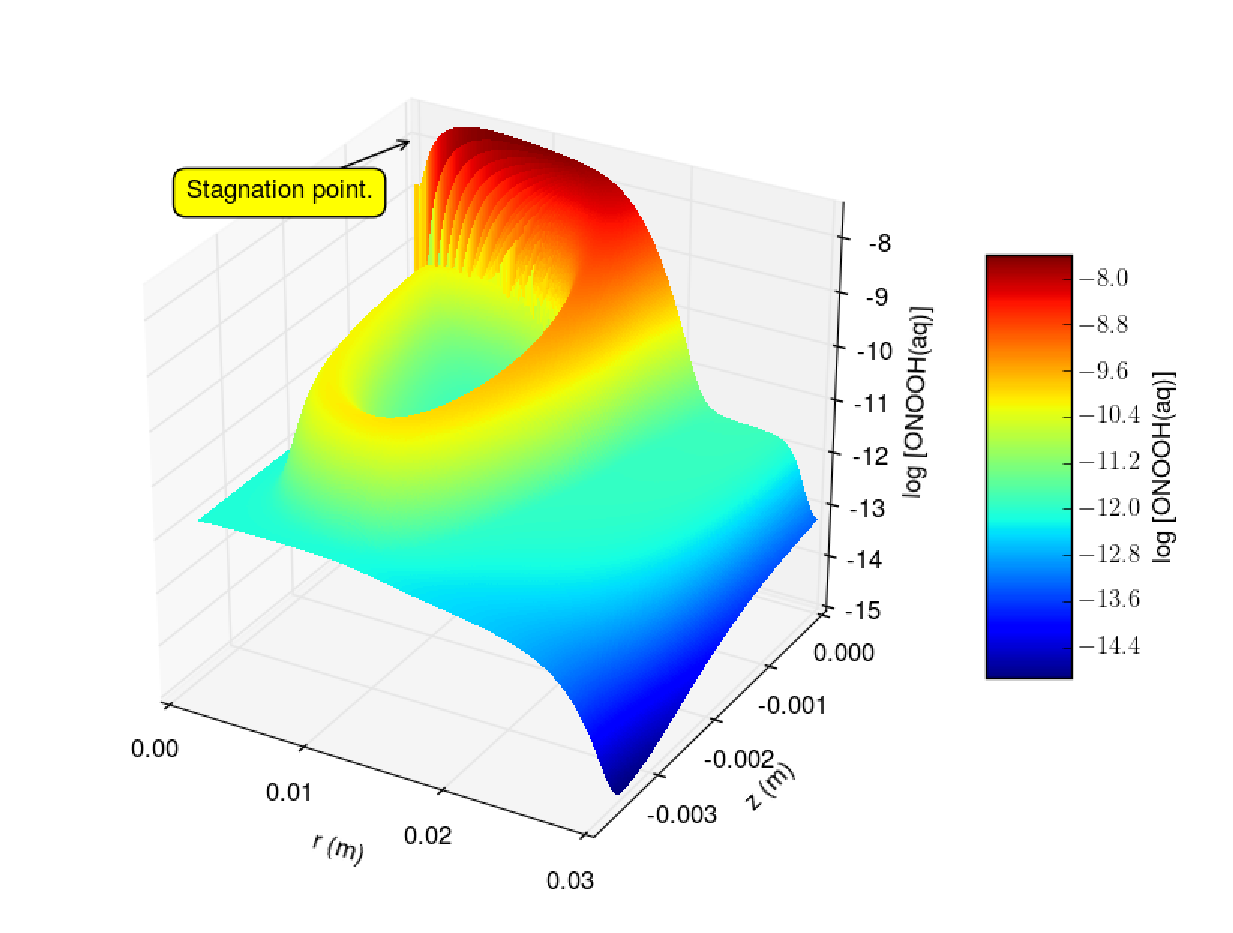
\includegraphics[width=\textwidth]{logONOOH.eps}
    \caption{3D plot of log$_{10}$(ONOOH(aq)) as a function of position for t = 1000 seconds. As with OH, large interfacial gradients are evident as is the effect of the liquid convection loop. Note that the r and z axes have different scales}
    \label{fig:log_ONOOH_conc}
\end{figure}

\begin{figure}[htb]
    \centering
    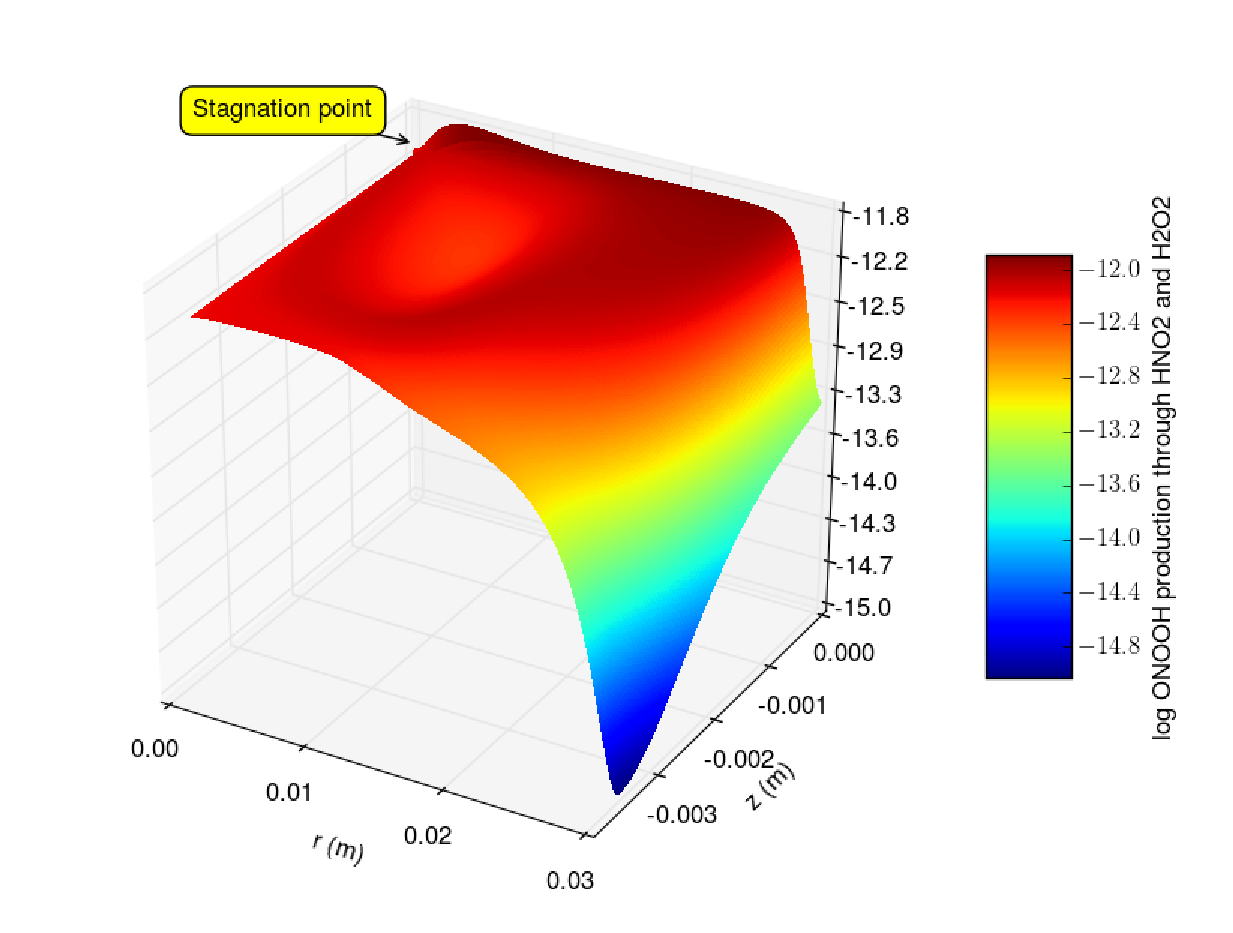
\includegraphics[width=\textwidth]{logONOOHproduced.eps}
    \caption{3D plot of the base 10 logarithm of the producation rate of ONOOH through reaction \ONOOHlong{} listed in table \ref{tab:rxns}. Because of the relative uniformity in the distribution of H$^+$, H$_2$O$_2$, and NO$_2^-$, the production of ONOOH through reaction \ONOOHlong{} is much more uniform than the overall concentration profile of ONOOH. Note that the r and z axes have different scales.}
    \label{fig:log_ONOOH_prod_rate}
\end{figure}

The results presented here suggest two different regimes of activity in the solution: surface and bulk. When the discharge is on, reactivity in the form of OH is confined almost entirely to the plasma-liquid interface. Bulk solution concentrations of OH are several orders of magnitude lower than the surface concentration. This is also true of other potentially biologically important and highly reactive reagents such as NO and NO$_2$ radicals. Less reactive plasma-generated RONS like H$_2$O$_2$ and NO$_2^-$ have significantly longer lifetimes and can be transported into the bulk solution where they can react and form ONOOH, a precursor to OH and NO$_2$. However, for the model inputs used here, the bulk reactivity generated through H$_2$O$_2$ and NO$_2^-$ precursors is orders of magnitude less on a per unit time scale than the surface reactivity coming from direct fluxes of plasma generated radicals. When the discharge is turned off, generation of reactive species through H$_2$O$_2$ and NO$_2^-$ will persist for a while in the bulk. The results in \cite{Lukes2014b} show a nitrite half-life of 2-3 hours in acidic solution; Traylor et. al. \cite{Traylor2011h} observed anti-bacterial efficacy of PAW, which they attributed to ONOOH and its products, for several days after plasma treatment. If one assumes that every mole of H$_2$O$_2$ present in solution at the conclusion of our simulation reacts over time to form ONOOH and 30\% of ONOOH dissociation creates OH, then the amount of OH coming from this long-term bulk reaction is 32\% less than the amount of OH that comes from surface fluxes while the ``discharge" is on. This comparison suggests that if one is willing to wait many hours or several days, bulk reactivity can approach surface reactivity on an order of magnitude scale. However, if an application demands speed and efficient utilization of plasma generated reactivity, the target must be placed right at the plasma-liquid interface. If the target is removed from the plasma by millimeters or even hundreds of $\mu$m of aqueous solution, its rate of treatment will rely on a serial process: the rate of transport of longer-lived species like H$_2$O$_2$ and NO$_2^-$ through the bulk fluid followed by the rate of formation of peroxynitrous acid chemistry.

It should be noted that aqueous phase specie concentrations will be a function of plasma conditions such as electric field distribution and as previously mentioned, the water vapor concentration in the plasma region. Water vapor concentration will play a large role in determining the gas phase concentrations of species such as OH and H$_2$O$_2$. For a geometric configuration similar to that modelled here, Yagi, et. al. \cite{yagi2015two} showed relative humidity in the vicinity of the plasma increasing from less than 5\% to 90\% as the flow rate was decreased from 1 to 0.05 liters per minute (Lpm). Decreased water vapor content led to a significant reduction in gas phase OH for flow rates as low as 0.3 Lpm, which is comparable to the flow rate in this study. Since the gas phase inputs for the model were taken from a DBD configuration, it seemed prudent to consider whether the likely reduced fluxes of water vapor delivered to the gas-liquid interface in a jet or streamer-type system would affect one of the principal qualitative conclusions of this study: that aqueous bulk concentrations of highly reactive radicals can be orders of magnitude less than their interfacial concentrations.

To study this, we constructed a 1D model of just the liquid phase, neglecting liquid-phase convection (mostly in the radial direction at the interface) and considering only diffusion and reaction. Steady-state interfacial concentrations of OH, NO, NO$_2$, and N$_2$O$_4$ from the full 2D axisymmetric simulation were scaled up by a factor of ten and used as boundary conditions in the 1D liquid model. The scaling in the 1D model is meant to produce conditions more comparable to those in experiments. Using the described boundary conditions, the penetration distances of OH and NO into the bulk solution (defined to be the distance required for a log reduction in concentration) were 5.8 and 4.7 $\mu$m respectively. Another simulation was conducted in which the interfacial concentration of OH was reduced by a factor of 10 to reflect the potential reduction in OH fluxes to the interface for convective discharge systems. Under this scenario, OH and NO penetration distances were both 16$\mu$m. In both simulations, NO$_2$ concentrations fell sharply in the first tens of microns but then displayed a second local concentration maximum around 100 $\mu$m. This second concentration maximum arises from ONOOH dissociation rates outweighing the loss of NO$_2$ through radical reactions; as already stated, two of NO$_2$'s principal reaction partners, NO and OH, are depleted within the first tens of microns. The concentration of NO$_2$ at this second maximum is an order of magnitude less than the interfacial NO concentration and two orders of magnitude less than the interfacial OH concentration for the diluted convective case. If the OH concentration were diluted quite a bit further (which may not be physically realistic), it is conceivable that NO penetration as predicted by our model could approach hundreds of microns or even millimeters. However, the physical conditions that would promote a very low interfacial OH concentration may also promote higher NOx radical interfacial concentrations than those used in our model. NOx radical reaction rate constants are on the same order of magnitude as OH reactions (~1e10 moles/L); consequently one could envision a case in which interfacial OH radical concentrations are very low, but the penetration distance of radical NOx species is still on the order of microns because of self-reactions.

On a related note, the 1D model can be used to analyze the effect of the uniform dilution factor used in the 2D-axisymmetric model on the penetration distance of radicals. From the species mass conservation equations we expect penetration distances to decrease as input concentrations are scaled up since the only non-linear terms are reaction sinks. More precisely, the dimensionless Damkohler number, $Da=\frac{kCL^2}{D}$, for a second-order reaction-diffusion problem shows that the penetration distance will scale like $\frac{1}{\sqrt{C}}$. \cite[p. 55]{deen1998analysis} This hypothesis is confirmed by the 1D model. When the interfacial concentrations from the 2D-axisymmetric model are input directly into the 1D model, OH and NO penetration distances are 18 and 15 microns respectively. These are almost exactly a factor of $\sqrt{10}$ greater than the 5.8 and 4.7 $\mu$m penetration distances seen when the concentration inputs are scaled up by 10. If the concentrations are increased more, the penetration distances are even further reduced, following the scaling of $\frac{1}{\sqrt{C}}$. These analyses of the radical concentration profiles support one of our main arguments: though the amount and type of species present at the plasma-liquid interface may vary between discharge types, most of the plasma generated reactivity will likely lie within a small interfacial region, microns to a couple hundred microns, regardless of the experimental configuration.

Returning to the 2D model, we can introduce a dissolved marker like Tyrosine into solution and observe its degradation via reactive plasma species and predict product formation for potential future validation with experiments. \Cref{fig:tyr_conc} shows the concentration profile of tyrosine after fifteen minutes of exposure to reactive plasma species. The origin represents the stagnation point or the point at which the center of the plasma column impinges on the liquid surface. Z = 0 represents the water surface. After treatment, the concentration of tyrosine at the surface has been roughly cut in half. The presence of bulk liquid advection is evident in the decreased tyrosine concentration surrounding a local maximum at roughly (.01, -.0015). We can also look at the volume-averaged concentrations of tyrosine products in \cref{fig:tyr_products}. TyrDot is tyrosine radical, diTyr is dityrosine, TyrNO is tyrosine with an added NO functional group, TyrNO2 has an added NO$_2$ functional group, and TyrOHo and TurOHm are tyrosine with an additional OH functional group at the ortho- and meta- positions respectively. Our model predicts that dityrosine will be the dominant terminal specie with TyrOHm and TyrDot representing important reactive intermediates.

\begin{figure}[htb]
    \centering
    \includegraphics[width=\textwidth]{tyrosine_products.png}
    \caption{Plot vs. time showing the growth of different tyrosine products. The dominant product formed is dityrosine.}
    \label{fig:tyr_products}
\end{figure}

\begin{figure}[htb]
    \centering
    \includegraphics[width=\textwidth]{tyrosine_conc.png}
    \caption{Plot of tyrosine concentration at the end of 15 minutes of reactive species exposure. Concentration is significantly depleted near the liquid surface as well as within the advective re-circulating loop.}
    \label{fig:tyr_conc}
\end{figure}

\begin{figure}[htb]
    \centering
    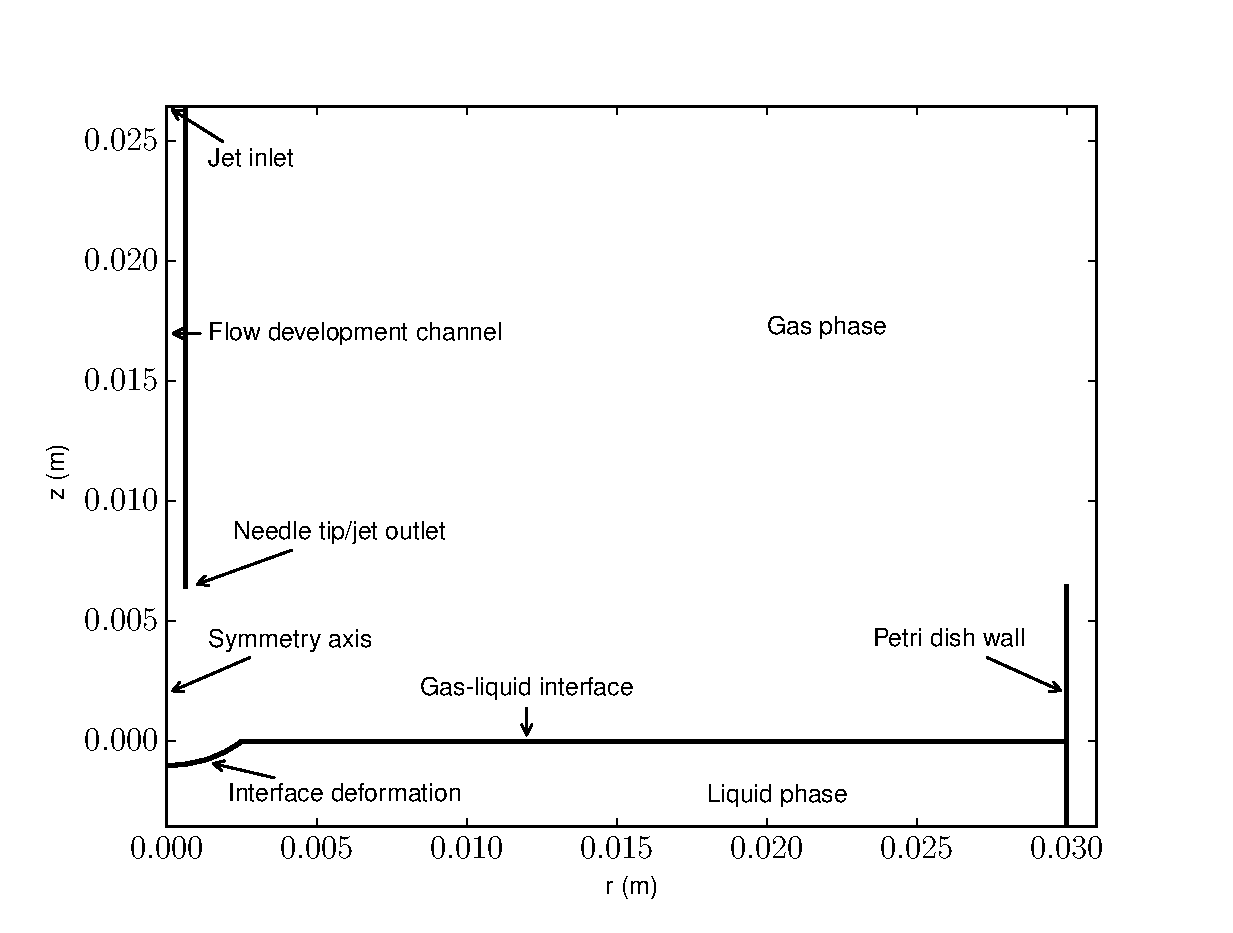
\includegraphics[width=\textwidth]{GeometryDeformed.eps}
    \caption{Geometry for deformed interface simulations.}
    \label{fig:deformed_geom}
\end{figure}

\begin{figure}[htb]
    \centering
    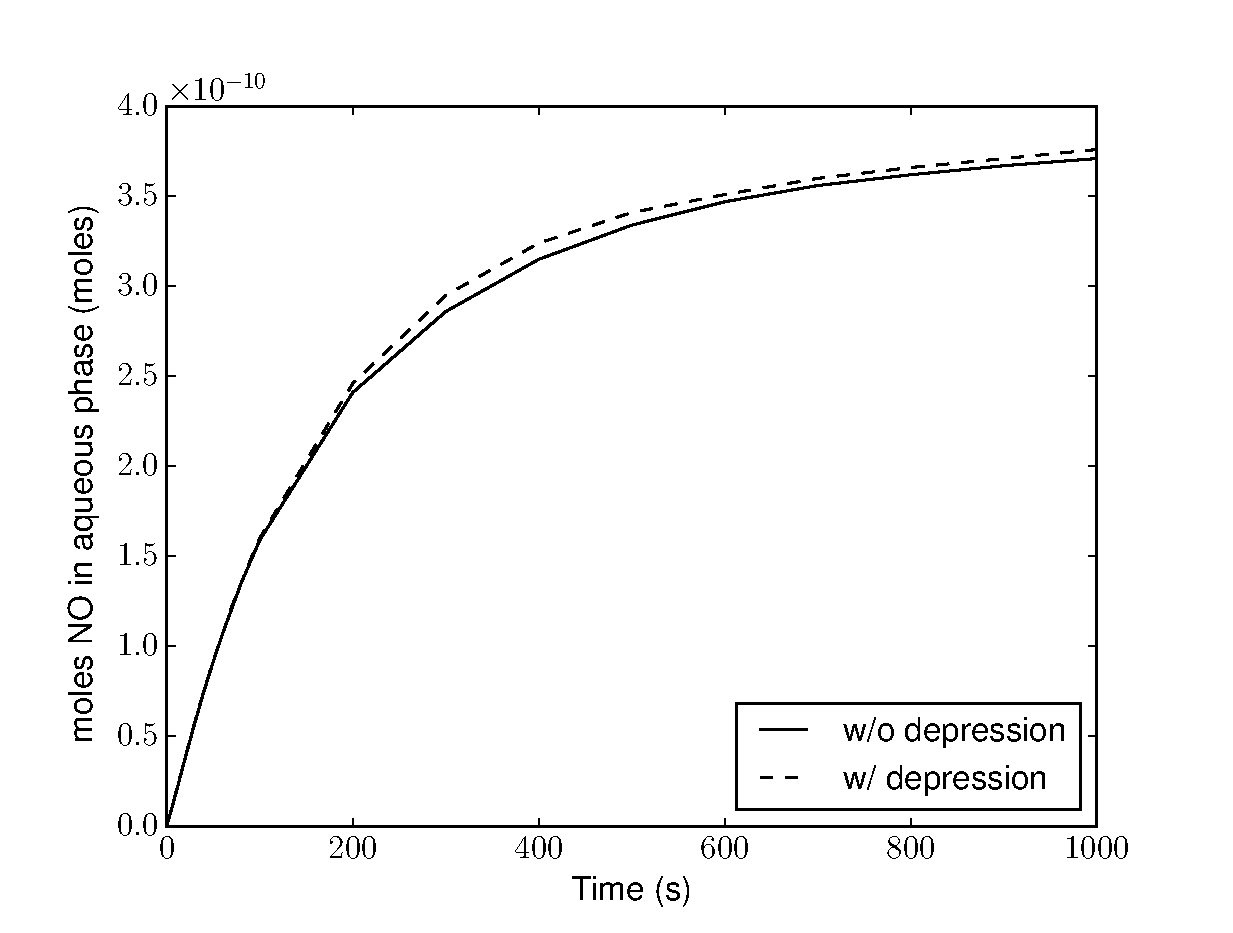
\includegraphics[width=\textwidth]{NO_dimple_plot.eps}
    \caption{Comparison of total NO(aq) uptake as a function of time for cases in which interface deformation is included and not included. As shown in the figure, the interface deformation has very little effect on the macrosocpic NO uptake. The effect for hydrophilic species is expected to be even less}
    \label{fig:NO_deform_compare}
\end{figure}

Before concluding, it is worth touching on the assumption of a flat interface. This work discusses the role gas phase convection plays in determining momentum, heat, and mass transport across a gas-liquid interface and into the bulk liquid. Species uptake is used as the criteria for determining whether to include self-consistent deformation of the interface by the gas flow. To make this determination, the shape of the interface deformation was observed experimentally and the deformation was introduced into the model geometry as shown in figure \ref{fig:deformed_geom}. The depth of the deformation was supported by a calculation balancing gravitational ($\rho$gh) and convective ($\frac{1}{2}\rho$v$^2$) stresses. The fluid flow simulation was then run until it reached stead-state, and then the heat and mass transfer equations were solved. In this way, though the interface deformation was not self-consistently determined, its influence on variables of interest could be analyzed. Shown in \ref{fig:NO_deform_compare} is the effect of the interface deformation on total solution uptake of NO(aq). As can be seen in the figure, the effect is minute. Because of the characteristics shown in Figure \ref{fig:excel}, the effect of the interface deformation on hydrophilic species transport is expected to be even less. Subsequently, for the purpose of this work, the interface deformation can be safely neglected.

Though comprehensive in many respects, the model in this section is not near complete without simulation of plasma discharge physics. Incorporating discharge physics requires changing simulation platforms from Comsol to Zapdos, a highly customizable code built by the authors where near total control over solution of the highly-nonlinear plasma equations is maintained. Zapdos is described in detail in \cref{chap:zapdos}. The 1D simulation effort in \cref{sec:plasliq} are the authors' first foray into self-consistent discharge-liquid modelling. Along with exploring questions about interfacial parameters, the work in \cref{sec:plasliq} is absolutely necessary for extending the work in this section. Combining the two modelling efforts is definitely on the roadmap for future work.

\FloatBarrier

\section{Fully Coupled Simulation of the Plasma Liquid Interface and Interfacial Coefficient Effects}
\label{sec:plasliq}

\subsection{Model Description}
\label{sec:model}
../plasmaliq_paper/model_description.tex
\FloatBarrier

\subsection{Results and Discussion}
\label{sec:plasliq_results}
../plasmaliq_paper/results_discussion.tex

% Figures to add text for:

\begin{figure}[htpb]
  \centering
  \includegraphics[width=.75\textwidth]{dummy_PowerDep_em.eps}
  \caption{Power deposited in electrons near the interface as a function of the interfacial surface loss coefficient}
  \label{fig:powerDep_em_int}
\end{figure}

\Cref{fig:powerDep_em_int} shows the power deposited into electrons from Joule Heating over the last 100 $\mu$m of the gas domain. It is evident that there is significantly more heating of the electrons for the higher reflection cases. This is almost entirely attributable to the enhanced electric field in the region (\cref{fig:efield_int}) that develops because of the build-up in negative charge density (\cref{fig:charge_dens_int}) from electron reflection. The electron current itself does not change with reflection as evidenced in \cref{fig:currents}.

\begin{figure}[htpb]
  \centering
  \includegraphics[width=.75\textwidth]{InterfacialChargeDensity.eps}
  \caption{Charge density near the interface as a function of the interfacial surface loss coefficient}
  \label{fig:charge_dens_int}
\end{figure}

\begin{figure}[htpb]
  \centering
  \includegraphics[width=.75\textwidth]{ElectronIonPowerDepFullGasDomain.eps}
  \caption{Power deposited in ions and electrons over the whole gas domain for low and high reflection cases}
  \label{fig:powerDep_em_Arp_full}
\end{figure}

Power deposition into both electrons and ions for the cases of $\gamma_{dens}=1$ and $\gamma_{dens}=10^{-4}$ are shown in \cref{fig:powerDep_em_Arp_full}. Ion power deposition profiles are identical between the different reflection cases. As expected for a DC discharge, all of the ion power deposition occurs in the cathode fall where both the electric field and ion current are significantly higher than in the bulk. Electron heating occurs throughout the discharge with local maxima in both the cathode and anode regions.

\begin{figure}[htpb]
  \centering
  \includegraphics[width=.75\textwidth]{RateProcesses.eps}
  \caption{Rate of ionization, excitation, and elastic collisions in the plasma for low and high reflection cases}
  \label{fig:rateProc}
\end{figure}

\Cref{fig:rateProc} shows the rate of elastic, excitation, and ionization collisions in the discharge. Elastic collision rates show an inverse relationship to the electron temperature: in the cathode where the electron temperature peaks, the elastic collision rate crashes; in the anode for the high reflection case ($\gamma_{dens}=10^{-4}$) the elastic collision rate peaks sharply because of the sharp fall in the electron temperature. Excitation collision rates are uniform through the bulk of the discharge for both high and low reflecion cases. Ionization rates peak in the bulk-sheath interface regions where the electron temperature is highest. Both excitation and ionization rates collapse in the cathode where electrons have not had sufficient time to gain energy; for high electron reflection the excitation and ionization rates also collapse in the anode.

\begin{figure}[htpb]
  \centering
  \includegraphics[width=.75\textwidth]{Currents.eps}
  \caption{Plot of specie and total currents in gas and liquid phases for low and high reflection cases}
  \label{fig:currents}
\end{figure}

\Cref{fig:currents} is a somewhat busy figure. It illustrates the currents carried by different species in gas and liquid phases as well as the total current. Dotted lines indicate the total current, solid lines the electron current, and dashed lines the argon and hydroxyl currents in the gas and liquid phases respectively. The curves do not show a strong functional dependence on the surface loss coefficient $\gamma_{dens}$. Current is carried by argon ions in the cathode, transitioning to electrons in the gas bulk and through the gas-liquid interface. As electrons react with water molecules, OH$^-$ becomes the dominant liquid current carrier away from the interface.

\begin{figure}[htpb]
  \centering
  \includegraphics[width=.75\textwidth]{ElectronFluxesBothDomains.eps}
  \caption{Breakdown of electron diffusive and advective fluxes in both domains for low and high reflection cases}
  \label{fig:electron_fluxes}
\end{figure}

Electron total, advective, and diffusive fluxes are illustrated in \cref{fig:electron_fluxes}. Consistent with \cref{fig:currents}, the total electron current rises from zero at the cathode to a constant value that it maintains through the gas bulk to the interface. The total current declines in the liquid phase because of electron reactions with H$_2$O. Advection and diffusion flux profiles are very similar between high and low reflection cases with the exception of the behavior very near the gas-liquid interface. Advective flux builds in the cathode until reaching a peak at the sheath-bulk interface. The advective flux then gradually declines in the bulk because of a gradual decrease in the bulk electric field until plummeting sharply in the anode as the electron density plummets; however, for the high reflection case very near the gas-liquid interface the advective flux rebounds sharply. This counter-acts the very strong leftward diffusive flux that arises from the large build-up in electron concentration. The net effect is that the total electron flux remains constant.

\section{Summary}

This chapter addresses a couple of fundamental questions regarding plasma-liquids. A qualitative study of the momentum, heat, and mass transport in a convective plasma-liquid system has been conducted in \cref{sec:plasfree_model}. Several interesting results were found. Convective flow of water vapor away from the interface leads to a sharp temperature gradient between the bulk gas and liquid phases. This sharp gradient is important for accurately determining temperature-dependent rate coefficients in both the gas and liquid phases. Additionally, convection drives water vapor away from the discharge region except immediately above the liquid surface; this could have important consequences for gas-phase generation of reactive species that depend on water as a precursor. Induced convection in the liquid phase substantially changes the spatial distribution of aqueous species and increases the volume-averaged uptake of hydrophobic species but interestingly has little effect on the volume-averaged uptake of hydrophilic species. This phenomena occurs because the majority of resistance to interfacial transfer is in the gas phase for hydrophilic species and in the liquid phase for hydrophobic species; consequently, decreasing the liquid-phase mass transfer resistance by adding liquid convection has a significant impact for hydrophobic but not for hydrophilic molecules.

Perhaps the most interesting result of the study in \cref{sec:plasfree_model} is the sharp distinction between reactivity at the surface and in the liquid bulk. Though the limited penetration (tens of $\mu$m or less) of reactive neutral radicals is well publicized in prominent biochemistry texts like \cite{Halliwell}, this phenomena has yet to receive significant attention in the plasma-liquid literature with the exception of \cite{Chen2014a}. Concentrations of species of interest for plasma-medicine and other applications (e.g. OH, NO, ONOOH) fall by as many as 9 orders of magnitude within 50 $\mu$m of the interface. In a relatively pure aqueous solution as is modeled here, the process responsible for conveying plasma reactivity to a target may be transport of H$_2$O$_2$ and acidified nitrite followed by a close-proximity reaction to form ONOOH and then OH and NO$_2$. For targets in aqueous biological systems, the conveyors of reactivity may be proteins modified by primary plasma species. What can be stated from the results presented here and in \cite{Chen2014a} is that these conveyors of plasma reactivity are probably not neutral radicals generated directly by the plasma; rather they are likely species generated by secondary reactions in the aqueous medium or more stable compounds like H$_2$O$_2$ and nitrite. To address this problem with even greater precision and detail, future research will involve developing a configuration-specific plasma and electrodynamics model that can be self-consistently coupled to the momentum, heat, and neutral species mass transport presented in this study.

The latter half of the chapter explores the fully self-consistent coupling of discharge physics with the liquid phase. The effects of varying unknown interfacial coefficients like $\gamma_{dens}$ and $\gamma_{en}$ are investigated. It is found that varying these parameters within reason can lead to interfacial gas-phase electron densities varying by orders of magnitude. The interfacial electron energy is also a very sensitive function of the interfacial parameters. This variation of electron density and energy could have significant impacts on both gas and liquid phase chemistry, thus our work motivates future studies to accurately determine the interfacial parameters. It is noteworthy that the overall potential drop and total current are relatively unaffected by changing gas-liquid interfacial parameters.

Self-consistently coupling the liquid domain to the highly non-linear plasma discharge equations as is done for \cref{sec:plasliq} requires an efficient multi-physics code. Comsol, the package used for the simulations in the first half of \cref{chap:basic_science}, has typically struggled to efficiently solve plasma problems. Thus a new code, named Zapdos, was built on top of the MOOSE framework for the express purpose of plasma-liquid simulations (although the highly modular nature of the code makes it easily extensible to other low-temperature plasma problems). The structure of Zapdos is the subject of \cref{chap:zapdos}.
